% \documentclass[amsmath, amssymb]{revtex4}
% \documentclass[dvips,aoas,preprint]{imsart}
\documentclass[aoas,preprint]{imsart}
% \documentclass{article}
% \input{/Users/joshyv/Research/misc/latex_paper.tex}
%\documentclass[11pt]{article}
\usepackage{a4wide}
\usepackage{apalike}
\usepackage{algorithm}
\usepackage{algpseudocode}
\usepackage{graphicx}% Include figure files
\usepackage{amsmath}
\usepackage{amsfonts}
\usepackage{amsthm}
% \usepackage{charter}
% \usepackage{afterpage}
% \usepackage{cite}
% \usepackage{algorithmic}

%\usepackage{dcolumn}% Align table columns on decimal point
%\usepackage{bm}% bold math
% \RequirePackage[OT1]{fontenc}
% \RequirePackage{amsthm,amsmath,natbib}
%\RequirePackage[colorlinks,citecolor=blue,urlcolor=blue]{hyperref}
% \RequirePackage{hypernat}

\startlocaldefs
\renewcommand{\i}{\backslash i}
\newcommand{\bth}{\mathbf{\theta}}
\newcommand{\w}{w}
\newcommand{\bw}{\mathbf{\w}}
\newcommand{\T}{^{\ensuremath{\mathsf{T}}}}           % transpose
\DeclareMathOperator*{\argmax}{argmax}
\DeclareMathOperator*{\argmin}{argmin}
\newcommand{\bF}{{\bf F}}
\newcommand{\bX}{{\bf X}}
\newcommand{\bn}{{\bf n}}
\newcommand{\bh}{\mathbf{h}}
\newcommand{\hbth}{\widehat{\bth}}
\newcommand{\tbth}{\tilde{\bth}}
\newcommand{\hbw}{\widehat{\bw}}
\newcommand{\sumit}{\sum_{\substack{i \in [1,\ldots,N] \\ t \in [1,\ldots, T]}}}
\long\def\comment#1{}

\endlocaldefs


\begin{document}
	
\begin{frontmatter}
\title{A Bayesian approach to inferring functional connectivity given population calcium imaging}
\runtitle{Inferring connectivity from calcium imaging}
% \thankstext{T1}{Footnote to the title with the `thankstext' command.}

\begin{aug}
\author{\fnms{Yuriy} \snm{Mishchencko}\thanksref{t1}\ead[label=e1]{y@somewhere.com}}
\author{\fnms{Joshua T.} \snm{Vogelstein}\thanksref{t2}\ead[label=e2]{joshuav@jhu.edu}},
\and
\author{\fnms{Liam} \snm{Paninski}\thanksref{t1}
\ead[label=e3]{liam@stat.columbia.edu}
\ead[label=u1,url]{http://www.foo.com}}

\thankstext{t1}{Department of Statistics and Center for Theoretical Neuroscience, Columbia University}
\thankstext{t2}{Johns Hopkins University}
% \thankstext{t3}{Second supporter of the project}
\runauthor{Y. Mishchenko et al.}

% \affiliation{Some University\thanksmark{m1} and Another University\thanksmark{m2}}

\address{Yuriy Mishchenko\\
city street in turkey\\
\printead{e1}\\
% \phantom{E-mail:\ }\printead*{e1}
}

\address{Joshua Vogelstein\\
Johns Hopkins University\\
3400 N. Charles St.\\
Baltimore, MD, 21205 \\
\printead{e2}\\
% \printead{u1}
}

\address{Liam Paninski\\
address\\
usually few lines long\\
\printead{e3}\\
\printead{u1}}

\end{aug}

\begin{abstract}
Deducing the structure of neural circuits from neural activity is one of the central problems of modern neuroscience. Recent studies have examined this problem by observing neural activity  of dozens of neurons using multi-electrode techniques. Here, we present a model-based optimal approach for inferring the structure of neural micro-circuits containing hundreds of neurons observed with calcium imaging. While calcium imaging allows less intrusive observations of neural activity in potentially much larger populations than multi-electrode techniques, it provides only indirect observations of neural spike trains, which often may have limited time resolution and signal quality.  To infer the functional connectivity matrix of neural micro-circuits from such indirect data, we assume each observable neuron can accurately be described by a generalized linear model, forming a coupled hidden-Markov model for the whole network. The sufficient statistics of the cross-coupling terms --- i.e. the functional connectivity matrix --- are obtained using an embedded-chain-within-blockwise-Gibbs algorithm, which produces samples of joint spike trains of all observed neurons given the calcium traces. By introducing a factorized approximation for the likelihood of such joint spike trains, we are able to implement our algorithm in parallel on a high-performance cluster, without a significant degradation of inference results.  Imposing biophysically realistic constraints on our model, such as a sparseness of the connectivity matrix, facilitates a great reduction in the amount of data required to obtain a good fit.  Thus, using realistic simulations of spontaneous activity in populations of randomly connected neurons, we show that this method can successfully infer the connectivity patterns from $\approx 10$ minutes of calcium imaging data for neural populations up to $500$ neurons large, in approximately $10$ minutes of computational time.  Further, we show that this approach is robust to certain reasonable model misspecifications.
\end{abstract}

\begin{keyword}[class=AMS]
\kwd[Primary ]{60K35}
\kwd{60K35}
\kwd[; secondary ]{60K35}
\end{keyword}

\begin{keyword}
\kwd{Bayesian inference}
\kwd{Metropolis}
\kwd{MCM}
\kwd{causality}
\end{keyword}

\end{frontmatter}
	

\section{Introduction}
\label{intro}
Since Ramon y Cajal discovered that the brain is a rich and dense network of neurons \cite{RamonyCajal04,RamonyCajal23}, neuroscientists have been intensely curious about the details of these networks, which are believed to be the biological substrate for memory, cognition, and perception. While we have learned a great deal in the last century about ``macro-circuits'' (the connectivity between coarsely-defined brain areas) relatively little is known about ``micro-circuits,'' i.e., the connectivity within populations of neurons at a fine-grained cellular level. One can imagine two complementary strategies for inferring micro-circuits: anatomical and functional. Anatomical approaches to inferring circuitry do not rely on observing neural activity.  Several interesting anatomical strategies are being pursued by other groups , such as array tomography \cite{MichevaSmith07}, ``brainbow'' mice \cite{Brainbow07}, and serial electron microscopy \cite{Briggman2006}. Our work,  takes a functional approach: our aim is to infer micro-circuits by observing only the activity of a population of neurons, and not any neural processes.

Experimental tools that enable approximately simultaneous observations of the activity of many (e.g., $O(10^3)$) neurons are now widely available. While arrays of extracellular electrodes have been exploited for this purpose, the arrays most often used \emph{in vivo} are inadequate for inferring monosynaptic connectivity in very large populations of neurons, as the inter-electrode spacing is typically too large to record from neighboring neurons, and number of electrodes in the arrays limits the number of neurons that can be simultaneously observed \cite{HATS98,HARR03,Stein04,Santhanam06,Harris07}\footnote{It is worth noting, however, that multielectrode arrays which have been recently developed for use in the retina are capable of much denser sampling \cite{Berry2004,Litke2004,Petrusca07,PILL07}.}. Alternately, calcium-sensitive fluorescent indicators facilitates observing the spiking activity of up to $O(10^4)$ neighboring neurons \cite{Tsien89,ImagingManual}.  Importantly, neighboring neurons are more likely connected to one another than than distant neurons \cite{Abeles91,Braitenberg1998}. Some organic dyes achieve sufficiently high signal-to-noise ratios (SNR) that individual action potentials (spikes) may be resolved \cite{ImagingManual}, and bulk-loading techniques enable experimentalists to simultaneously fill populations of neurons with such dyes \cite{StosiekKonnerth03}. In addition, genetically encoded calcium indicators are under rapid development in a number of groups, and are approaching SNR levels of nearly single spike accuracy as well \cite{WallaceHasan08}. Microscopy technologies for collecting fluorescence signals are also rapidly developing. Cooled CCDs for wide-field imaging (either epifluorscence or confocal) now achieve a quantum efficiency of $\approx 90 \%$ with frame rates up to $60$ Hz or greater, depending on the field of view \cite{Djurisic04}. For in vivo work, 2-photon laser scanning microscopy can achieve similar frame rates, using either acoustic-optical deflectors to focus light at arbitrary locations in three-dimensional space \cite{ReddySaggau05,Iyer06,SalomeBourdieu06,ReddySaggau08}, or resonant scanners \cite{NguyenParker01}. Together, these experimental tools can provide movies of calcium fluorescence transients for small populations of neurons (e.g., $O(10^2)$) with ``reasonable'' SNR, and at imaging frequencies of $30$ Hz or greater, in both the in vitro and in vivo settings.

Given these experimental advances in functional neural imaging, our goal is to develop efficient computational and statistical methods to exploit this data for the analysis of neural connectivity (see Figure \ref{fig:data_schematic} for a schematic overview). One major challenge here is that calcium transients due to action potentials provide indirect observation of the neural activity, and decay about an order of magnitude slower than the time course of the underlying neural activity \cite{ImagingManual}. Thus, to properly analyze the functional network connectivity, we must incorporate a method for effectively deconvolving the observed noisy fluorescence signal to obtain estimates of the underlying spiking rates \cite{YaksiFriedrich06,GreenbergKerr08,Vogelstein2009}. To this end we introduce a coupled Markovian state-space model that relates the observed variables (fluorescence traces from the neurons in the microscope's field of view) to the hidden variables (spike trains and intracellular calcium concentrations of these neurons), as governed by a set of biophysical parameters including the network connectivity matrix. Given this model, we derive a Monte Carlo Expectation Maximization algorithm for obtaining the maximum a posteriori estimates of the parameters of interest. Standard Monte Carlo sampling procedures (e.g., Gibbs sampling or sequential Monte Carlo) are inadequate in this setting, due to the high dimensionality and non-linear, non-Gaussian dynamics of the hidden variables in our model; we therefore develop a specialized blockwise-Gibbs approach to overcome these obstacles. This strategy enables us to accurately infer the functional connectivity matrix from large simulated neural populations, under realistic assumptions about the dynamics and observation parameters. We describe our approach below, along with several methods for improving its computational speed and statistical efficiency.

\section{Methods}
\label{sec:methods}
\subsection{Model}
\label{sec:methods:markov-setup}

We begin by detailing a parametric generative model for the (unobserved) joint spike trains of all $N$ observable neurons, along with the observed calcium fluorescence data. Each neuron is modeled as a generalized linear model (GLM). This class of models is known to capture the statistical firing properties of individual neurons fairly accurately \cite{BRIL88,CSK88,BRIL92,PG00,PILL07,PAN03d,PAN04c,Rigat06,TRUC05,NYK06,KP06,Vidne08,Stevenson2009}. We denote the $i$-th neuron's activity at time $t$ as $n_i(t)$: in continuous time, $n_i(t)$ could be modeled as an unmarked point process, but we will take a discrete-time approach here, with each $n_i(t)$ taken to be a binary random variable. We model the spiking probability of neuron $i$ via an instantaneous nonlinear function, $f(\cdot)$, of the filtered and summed input to that neuron at that time, $J_i(t)$. This input is composed of: (i) some baseline value, $b_i$; (ii) some external vector stimulus, $S^{ext}(t)$, that is linearly filtered by $k_i$; and (iii) spike history terms, $h_{ij}(t)$, encoding the influence on neuron $i$ from neuron $j$, weighted by $\w_{ij}$:
\begin{equation} \label{eqn:glm:definition}
\begin{array}{l}
n_i(t) \sim \text{Bernoulli}\left[f\left(J_i(t) \right) \right], \qquad
J_i(t)=b_i+k_i\cdot S^{ext}(t)+\sum \limits_{j=1}^{N} \w_{ij} h_{ij}(t).
\end{array}
\end{equation}

To ensure computational tractability of the parameters inference problem, we must impose some reasonable constraints on the instantaneous nonlinearity $f(\cdot)$ (which plays the role of the inverse of the link function in the standard GLM setting) and on the dynamics of the spike-history effects $h_{ij}(t)$. First, we restrict our attention to functions $f(\cdot)$ which ensure the concavity of the spiking loglikelihood in this model \cite{PAN04c,Escola07}, as we will discuss at more length below. In this paper, we use
\begin{equation}
f(J) = P\left[n>0 ~|~ n \sim \text{Poiss}\left(e^J\Delta\right)\right] = 1 - \exp[-e^J \Delta]
\end{equation}
(Figure \ref{fig:egfluor}), where the inclusion of $\Delta$, the time step size, ensures that the firing rate scales properly with respect to the time discretization; see \cite{Escola07} for a proof that this $f(\cdot)$ satisfies the required concavity constraints. However, we should note that in our experience the results depend only weakly on the details of $f(\cdot)$ within the class of log-concave models \cite{LD89,PAN04c}.

\begin{figure}[t!]
\centering 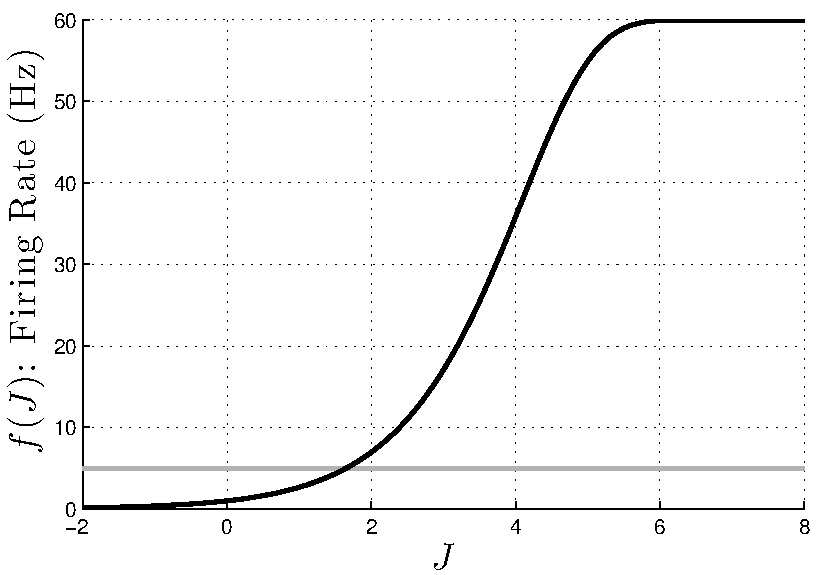
\includegraphics[width=3in]{../figs/fr_vs_J}
\caption{A plot of the firing rate nonlinearity $f(J)$ used in our
  simulations.  Note that the firing
  rate saturates at $1/\Delta$, because of our Bernoulli assumption
  (i.e., the spike count per bin is at most one). Here $\Delta = (60$
  Hz$)^{-1}$.}
\label{fig:egfluor}
\end{figure}

Second, because the algorithms we develop below assume Markovian dynamics, we model the spike history terms as an autoregressive process:
\begin{equation} \label{eqn:h:definition}
h_{ij}(t) = (1- \Delta/\tau^h_{ij}) h_{ij}(t- \Delta) +n_j(t) + \sigma^h_{ij}
  \sqrt{\Delta} \epsilon^h_{ij}(t),
\end{equation}
where $\tau^h_{ij}$ is the decay time constant for spike history terms, $\sigma^h_{ij}$ is a standard deviation parameter, $\sqrt{\Delta}$ ensures that the statistics of this Markov process have a proper Ornstein-Uhlenbeck limit as $\Delta \to 0$, and throughout this paper, $\epsilon$ denotes an independent standard normal random variable. Note that this model generalizes (via a simple augmentation of the state variable $h_{ij}(t)$) to allow each neuron to have several spike history terms, each with a unique time constant, which when weighted and summed allow us to model a wide variety of possible post-synaptic effects, including bursting, facilitating, and depressing synapses; see \cite{Vogelstein2009} for further details. We restrict our attention to the case of a single time constant $\tau^h_{ij}$ per synapse here, so the deterministic part of $h_{ij}(t)$ is a simple exponential function. Furthermore, we assume that $\tau^h_{ij}$ is the same for all neurons and all synapses, although in principle each synapse could be modeled with its unique $\tau^h_{ij}$. We do that both for simplicity and also because we find that the detailed shape of the coupling terms $h_{ij}(t)$ had a limited effect on the inference of the connectivity matrix, as illustrated in Figure \ref{fig:vartau} below. Thus, we treat $\tau^h_{ij}$ and $\sigma^h_{ij}$ as known synaptic parameters which are the same for each neuron pair $(i,j)$, and denote them as $\tau_h$ and $\sigma_h$ hereafter.  We chose values for $\tau_h$ and $\sigma_h$ in our inference based on experimental data \cite{Lefort2009}. Therefore our unknown model spiking parameters are $\{\bw_i,k_i,b_i\}_{i\leq N}$, with $\bw_i=(\w_{i1},\ldots, \w_{iN})$.

The problem of estimating the connectivity parameters $\bw=\{\bw_i\}_{i\leq N}$ in this type of GLM, given a fully-observed ensemble of neural spike trains $\{n_i(t)\}_{i\leq N}$, has recently received a great deal of attention; see the references above for a partial list. In the calcium fluorescent imaging setting, however, we do not directly observe spike trains; $\{n_i(t)\}_{i\leq N}$ must be considered a hidden variable here. Instead, each spike in a given neuron leads to a rapid increase in the intracellular calcium concentration, which then decays slowly due to various cellular buffering and extrusion mechanisms. We in turn make only noisy, indirect, and subsampled observations of this intracellular calcium concentration, via fluorescent imaging techniques \cite{ImagingManual}. To perform statistical inference in this setting, \cite{Vogelstein2009} proposed a simple conditional first-order hidden Markov model (HMM) for the intracellular calcium concentration $C_i(t)$ in cell $i$ at time $t$, along with the observed fluorescence, $F_i(t)$:
\begin{align}
\label{eqn:ca:definition}
C_i(t) &= C_i(t-\Delta) + (C_i^b-C_i(t-\Delta)) \Delta/\tau^c_i + A_i
n_i(t)+\sigma^c_i \sqrt{\Delta} \epsilon^c_i(t), \\ F_i(t) &= \alpha_i
S(C_i(t)) + \beta_i + \sqrt{\gamma_i S(C_i(t)) + \sigma^F_i}
\epsilon^F_i(t). \label{eqn:F:definition}
\end{align}
This model can be interpreted as a simple driven autoregressive process: under nonspiking conditions, $C_i(t)$ fluctuates around the baseline level of $C_i^b$, driven by normally-distributed noise $\epsilon^c_i(t)$ with standard deviation $\sigma^c_i \sqrt{\Delta}$. Whenever the neuron fires a spike, $n_i(t)=1$, the calcium variable $C_i(t)$ jumps by a fixed amount $A_i$, and subsequently decays with time constant $\tau^c_i$. The fluorescence signal $F_i(t)$ corresponds to the count of photons collected at the detector per neuron per imaging frame. This photon count may be modeled with normal statistics, with the mean given by a scaled and shifted Hill function $S(C)=C/(C+K_d)$ \cite{Yasuda2004} and the variance proportional to the mean (which follows from assuming the Poisson statistics of the photon counts are well approximated with Normal distribution; see \cite{Vogelstein2009} for further discussion. Because the parameter $K_d$ effectively acts as a simple scale factor, and is a property of the fluorescent indicator, we assume throughout this work that it is known. Figure \ref{fig:example_traces} shows a couple examples depicting the relationship between spike trains and observations.

\begin{figure}
\centering
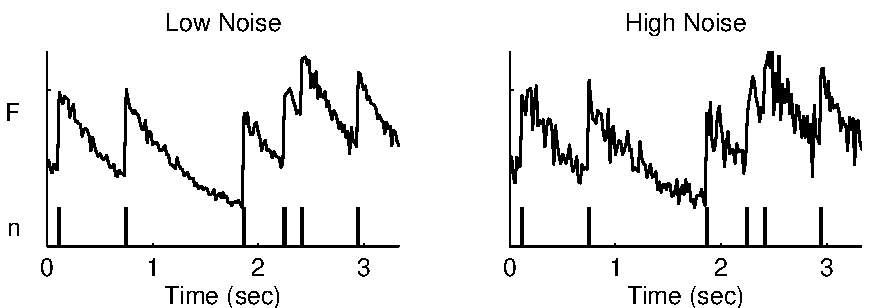
\includegraphics[width=\hsize]{../figs/sim_examples}
\caption{Both a low and high noise simulation showing typical relationships between spike trains and observations. Note that both panels have the same underlying spike train. Simulation parameters: $k_i=0.7$, $C_i^b=1$ $\mu$M, $\tau^c_i=500$ msec, $A_i=50$ $\mu$M, $\sigma^c_i=0.1$ $\mu$M,  $\alpha=2$, $\beta=0$, $\gamma=0.004, \, 0.016$ (left panel, right panel, respectively), $\sigma^F_i=0$.  $\Delta=1/60$ Hz.}
\label{fig:example_traces}
\end{figure}

To summarize, Eqs.~\eqref{eqn:glm:definition} -- \eqref{eqn:F:definition} define a coupled HMM: the underlying spike trains $\{n_i(t)\}_{i\leq N}$ and spike history terms $\{h_{ij}(t)\}_{i,j\leq N}$ evolve in a Markovian manner given the stimulus $S^{ext}(t)$. These spike trains in turn drive the intracellular calcium concentrations $\{C_i(t)\}_{i\leq N}$, which are themselves Markovian, but evolving at a slower timescale $\tau_i^c$. Finally, we observe only the fluorescence signals $\{F_i(t)\}_{i\leq N}$, which are related in a simple Markovian fashion to the calcium variables $\{C_i(t)\}_{i\leq N}$.

\subsection{Goal and general strategy}  \label{sec:methods:goal}

Our primary goal is to estimate the connectivity matrix, $\bw$, given the observed set of calcium fluorescence signals $\bF=\{\bF(t)\}_{t\leq T}$ and $\bF(t)=\{F_i(t)\}_{i\leq N}$. We must also deal with a number of nuisance parameters, $\tbth_i$: the intrinsic dynamics parameters $\{k_i, b_i, w_{ii}\}_{i\leq N}$, the calcium parameters $\{C^b_i, \tau^c_i, A_i, \sigma^c_i\}_{i\leq N}$, and the observation parameters $\{\alpha_i, \beta_i, \gamma_i, \sigma^F_i\}_{i\leq N}$. We addressed the problem of estimating these latter parameters in earlier work \cite{Vogelstein2009}; thus our focus here will be on the connectivity matrix $\bw$. A Bayesian approach is natural here, since we have a good deal of prior information about neural connectivity; see \cite{Rigat06} for a related discussion. However, a fully-Bayesian approach, in which we numerically integrate over the very high-dimensional parameters' space $\bth= \{\bth_i\}_{i\leq N}$, where $\bth_i=\{\bw_i, k_i, b_i, C^b_i, \tau^c_i, A_i, \sigma^c_i, \alpha_i, \beta_i, \gamma_i, \sigma^F_i\}$, is not particularly attractive from a computational point of view\footnote{The nuisance parameters for neuron $i$ are all its parameters, minus the cross-coupling terms, i.e.\ $\tbth_i =\bth_i \backslash \{w_{ij}\}_{i\neq j}$.}. Thus, our compromise is to compute \emph{maximum a posteriori} (MAP) estimates for the parameters via an expectation-maximization (EM) algorithm in which the sufficient statistics are computed by a hybrid blockwise Gibbs sampler and sequential Monte Carlo (SMC) method. More specifically, we iterate the steps:
\begin{align*}
\textbf{E step} &\text{: Evaluate } Q(\bth,\bth^{(l)}) = E_{P[\bX |
\bF; \bth^{(l)}]} \ln P \left[ \bF, \bX | \bth \right] = \int P[\bX |
\bF; \bth^{(l)}] \ln P[\bF, \bX | \bth] d \bX \\ \textbf{M step}
&\text{: Solve } \bth^{(l+1)} = \argmax_{\bth} \left\{
Q(\bth,\bth^{(l)}) + \ln P(\bth) \right\},
\end{align*}
where $\bX$ denotes the set of all hidden variables $\{ C_i(t), n_i(t), h_{ij}(t) \}_{i,j \leq N, t \leq T}$ and $P(\bth)$ denotes a (possibly improper) prior on the parameter space $\bth$. According to standard EM theory \cite{DLR77,McLachlanKrishnan96}, each iteration of these two steps is guaranteed to increase the log-posterior $\ln P(\bth^{(l)} | \bF)$, and will therefore lead to at least a locally maximum a posteriori estimator.

Now, our major challenge is to evaluate the auxiliary function $Q(\bth,\bth^{(l)})$ in the E-step. Our model is a coupled HMM, as discussed in the previous section; therefore, as usual in the HMM setting \cite{RAB89}, $Q$ may be broken up into a sum of simpler terms: 
\begin{eqnarray} 
Q(\bth,\bth^{(l)}) 
&=& \sum_{it} P[C_i(t) | F_i; \tbth_i] \times \ln P[F_i(t)|C_i(t); \alpha_i, \beta_i, \gamma_i, \sigma^F_i] \nonumber \\ 
&+& \sum_{it} P[C_i(t), C_i(t-\Delta), n_i(t) | F_i; \tbth_i] \times \ln P[C_i(t)|C_i(t-\Delta), n_i(t); C^b_i, \tau^c_i, A_i, \sigma^c_i] \nonumber \\ 
&+& \sum_{it} P[n_i(t), \bh_i(t) | \bF; \bth_i] \times \ln P[n_i(t)| \bh_i(t); b_i, k_i, \bw_i, S^{ext}(t)] 
% \nonumber \\
% &+& \sum_{it} P[h_i(t), h_i(t-\Delta),n_i(t) | F_i; \tbth_i] \times \ln P[h_i(t)| h_i(t-\Delta), n_i(t); \tau^h, \sigma^h], 
\label{eqn:loglik:definition-expl} 
\end{eqnarray} 
\noindent where $\bh_i(t)=\{h_{ij}(t)\}_{j \leq N}$. Note that each of the three sums here corresponds to a different component of the model described in Eqs.~\eqref{eqn:glm:definition} -- \eqref{eqn:F:definition}: the first sum involves the fluorescent observation parameters, the second the calcium dynamics, and the third the spiking dynamics (note the absence of a term for the spike history terms, as their parameters are assumed known a priori).

Thus we need only compute low-dimensional marginals of the full posterior distribution $P[\bX | \bF; \bth]$; specifically, we need pairwise marginals, of the form $P[C_i(t), C_i(t- \Delta) | F_i; \tbth_i]$, and marginals $P[C_i(t)|F_i;\tbth_i]$ and $P[n_i(t),\bh_i(t)|\bF;\bth_i]$. Details for calculating $P[C_i(t), C_i(t- \Delta) | F_i; \tbth_i]$ and $P[C_i(t)|F_i;\tbth_i]$ are found in \cite{Vogelstein2009}. Calculation of the joint marginal for high dimensional hidden variable $\bh_i$ necessitates the development of specialized blockwise Gibbs-SMC sampling method, as we describe in the subsequent sections \ref{sec:methods:indep} and \ref{sec:methods:joint}. Once we have obtained these marginals, the M-step breaks up into a number of independent optimizations that may be computed in parallel and which are therefore relatively straightforward (Section \ref{sec:methods:parameters HMM}); see section \ref{sec:methods:specific_implementation} for a pseudocode summary along with some specific implementation details.

\subsection{Initialization of nuisance parameters via sequential
  Monte Carlo methods} \label{sec:methods:indep}

We begin by constructing relatively cheap, approximate preliminary estimators for the nuisance parameters, $\tbth_i$.
%= \bth \backslash \{w_{ij}\}_{i\neq j}$, i.e., the observation parameters, $\{\alpha_i,\beta_i,\gamma_i,\sigma^F_i\}$, the calcium dynamics parameters $\{C^b_i,\tau^c_i, A_i, \sigma^c_i\}_i$, and the intrinsic spiking parameters, $\{k_i,b_i,w_{ii}\}$.
The idea is to initialize our estimator by assuming that each neuron is observed independently. Thus we want to compute $P[C_i(t), C_i(t-\Delta) | F_i; \tbth_i]$ and $P[C_i(t)|F_i;\tbth_i]$, and solve the M-step for each $\tbth_i$, with the connectivity matrix parameters held fixed. This single-neuron case is much simpler, and has been discussed at length in \cite{Vogelstein2009}; therefore, we only provide a brief overview here. The standard forward and backward recursions provide these posteriors \cite{ShumwayStoffer06}:
\begin{align}
% \hspace{-25mm}  
P[X_i(t) | F_i(0:t)] &\propto P[F_i(t)| X_i(t)] \int P[X_i(t) |
    X_i(t-\Delta)] P[X_i(t-\Delta) | F_i(0:t-\Delta)] dX_i(t-\Delta),
\label{eqn:forward} \\
% \hspace{-25mm} 
P[X_i(t), X_i(t-\Delta) | F_i] &= P[X_i(t) | F_i]
\frac{P[X_i(t) | X_i(t-\Delta)] P[X_i(t-\Delta) |
F_i(0:t-\Delta)]}{\int P[X_i(t) | X_i(t-\Delta)] P[X_i(t-\Delta) |
F_i(0:t-\Delta)] dX_i(t-\Delta)},
\label{eqn:backward}
\end{align}
where $F_i(s:t)$ denotes the time series $F_i$ from time points $s$ to $t$, and we have dropped the conditioning on the parameters for brevity's sake. Eq.~\eqref{eqn:forward} describes the forward (filter) pass of the recursion, and Eq.~\eqref{eqn:backward} describes the backward (smoother) pass, providing both $P[X_i(t), X_i(t-\Delta) | F_i]$ and $P[X_i(t)|F_i]$ (obtained by marginalizing by $X_i(t-\Delta)$).

Because these integrals cannot be analytically evaluated for our model, we approximate them using a SMC (``marginal particle filtering'') method \cite{DGA00,DFG01,GDW04}; see \cite{Vogelstein2009} for details on the proposal density and resampling methods used here. The output of this SMC method comprises an array of particle positions $\{X_i^{(m)}(t)\}_{m=1}^{M}$, where $m$ indexes the particle number, and a discrete approximation to the marginals $P[X_i(t), X_i(t-\Delta) | F_i]$,
\begin{multline}
% \begin{array}{rl}
P[X_i(t), X_i(t-\Delta) | F_i] \approx \\
\approx \sum_{m,m'}
r_i^{(m,m')}(t,t-\Delta) \delta \left[ X_i(t) - X_i^{(m)}(t) \right]
\delta \left[ X_i(t-\Delta) - X_i^{(m')}(t-\Delta) \right],
% \end{array}
\label{eqn:particle-fb}
\end{multline}
where $r_i^{(m,m')}(t,t-\Delta)$ denotes the weight attached to the
pair of particles with positions $\left( X_i^{(m)}(t),
X_i^{(m')}(t-\Delta) \right)$, and $\delta(.)$ denotes a Dirac mass.

As discussed above, the sufficient statistics for estimating the nuisance parameters for each neuron, $\tbth_i$, are exactly these marginal posteriors. As discussed following Eq.~\eqref{eqn:loglik:definition-expl}, the M-step decouples into three independent subproblems. The first term depends on only $\{\alpha_i, \beta_i, \gamma_i, \sigma_i\}$; since $P[F_i(t)|S(C_i(t)); \tbth_i]$ is quadratic (by our Gaussian assumption on the fluorescent observation noise), we can estimate these parameters by solving a weighted regression problem (specifically, we use a coordinate-optimization approach: we solve a quadratic problem for $\{\alpha_i, \beta_i\}$ while holding $\{\gamma_i, \sigma_i\}$ fixed, then estimate $\{\gamma_i,\sigma_i\}$ by the usual residual error formulas while holding $\{\alpha_i, \beta_i\}$ fixed). Similarly, the second term requires us to optimize over $\{\tau_i^c, A_i, C_i^b\}$, and then we use the residuals to estimate $\sigma_i^c$. Note that all the parameters mentioned so far are constrained to be non-negative, but may be solved efficiently using standard quadratic program solvers if we use the simple reparameterization $\tau_i^c \to 1- \Delta / \tau_i^c$. Finally, the last term, assuming neurons are independent, may be expanded:
\begin{multline}
E [\ln P[n_i(t), \bh_i(t) | \bF; \bth_i]] =  \\ = P[n_i(t), \bh_i(t) |
\bF] \ln f [J_i(t)] + (1-P[n_i(t), \bh_i(t) | \bF]) \ln [1-
f(J_i(t))];
\label{eqn:bw}
\end{multline}
since $J_i(t)$ is a linear function of $\{b_i,k_i,\bw_i\}$, and the right-hand side of Eq.~\eqref{eqn:bw} is concave in $J_i(t)$, we see that the third term in Eq.~\eqref{eqn:loglik:definition-expl} is a sum of terms which are concave in $\{b_i,k_i,\bw_i\}$ --- and therefore also concave in the linear subspace $\{b_i,k_i, w_{ii}\}$ with $\{w_{ij}\}_{i \neq j}$ held fixed --- and may thus be maximized efficiently using any convex optimization method, e.g.\ Newton-Raphson or conjugate gradient ascent.

Our procedure therefore is to initialize the parameters for each neuron using some default values that we have found to be practically effective in analyzing real data, and then recursively (i) estimate the marginal posteriors via Eq.~\eqref{eqn:particle-fb} (E step), and (ii) maximize the nuisance parameters $\tbth_i$ (M step), using the above described approach. We iterate these two steps until the change in $\tbth_i$ does not exceed some minimum threshold (or we reach an upper bound on iterations). We then use the marginal posteriors from the last iteration to seed the blockwise Gibbs sampling procedure described below. With that, we approximate $P[n_i,\bh_i | \bF;\bth_i]$.

\subsection{Estimating joint posteriors over weakly coupled neurons}
\label{sec:methods:joint}

Now we turn to the key problem: constructing an estimate of the joint marginals $\{P[n_i(t), \bh_i(t) | \bF;\bth]\}_{i\leq N}$, which are the sufficient statistics for estimating the connectivity matrix $\bw$ (recall Eq.~\eqref{eqn:loglik:definition-expl}). The SMC method described in the preceding section only provide the marginals over each neuron; this method may in principle be extended to obtain the desired full posterior $P[\bX(t), \bX(t-\Delta) | \bF; \bth]$, but the SMC is fundamentally a sequential importance sampling method, and therefore scales poorly as the dimensionality of the hidden state $\bX(t)$ increases \cite{BickelBengtsson08}. Thus we need a different approach.

One very simple idea is to use a Gibbs sampler: sample sequentially
from
\begin{align}
X_i(t) \sim P[X_i(t) | \bX_{\i}, X_i(0), \ldots, X_i(t-\Delta),
 X_i(t+\Delta), \ldots, X_i(T), \bF; \bth],
\end{align}
looping over all cells $i$ and all time bins $t$. Unfortunately, this approach is likely to mix poorly, due to the strong temporal dependence between $X_i(t)$ and $X_i(t+\Delta)$. Instead, we propose a blockwise Gibbs strategy, sampling one spike train as a block:
\begin{align}
	X_i \sim P[X_i | \bX_{\i}, \bF; \bth].
\end{align}
If we can draw these blockwise samples $X_i = X_i(s:t)$ efficiently for a large subset of $t-s$ adjacent time-bins simultaneously, then we would expect the resulting Markov chain to mix much more quickly than the single-element Gibbs chain.  This follows due to the weak dependence between $X_i$ and $X_j$ when $i\neq j$, and that Gibbs is most efficient for weakly-dependent variables \cite{RC05}.

So, how can we efficiently sample from $P[X_i | \bX_{\i}, \bF; \bth]$? One attractive approach is to try to re-purpose the SMC method described above, which is quite effective for drawing approximate samples from $P[X_i | \bX_{\i}, F_i; \bth]$ for one neuron $i$ at a time. Recall that sampling from an HMM is in principle easy by the ``propagate forward, sample backward'' method: we first compute the forward probabilities $P[X_i(t) | \bX_{\i}(0:t), F_i(0:t); \bth]$ recursively for timesteps $0$ up to $T$, then sample backwards from $P[X_i(t) | \bX_{\i}(0:T), F_i(0:T), X_i(t-\Delta); \bth]$. This approach is powerful because each sample requires just linear time to compute (i.e., $O(T/\Delta)$ time, where $T/\Delta$ is the number of desired time steps). Unfortunately, in this case we can only compute the forward probabilities approximately (with the SMC forward recursion approximation to Eq.~\eqref{eqn:forward}), and so therefore this attractive forward-backward approach only provides approximate samples from $P[X_i | \bX_{\i}, \bF; \bth]$, not the exact samples required for the validity of the Gibbs method.

Of course, in principle we should be able to use the Metropolis-Hastings (M-H) algorithm to correct these approximate samples. The problem is that the M-H acceptance ratio in this setting involves a high-dimensional integral over the set of paths that the particle filter might possibly trace out, and is therefore difficult to compute directly. \cite{Andrieu2007} discuss this problem at more length, along with some proposed solutions. A slightly simpler approach was introduced by \cite{NBR03}. Their idea is to exploit the $O(T/\Delta)$ forward-backward sampling method by embedding a discrete Markov chain within the continuous state space $\mathcal{X}_t$; the state space of this discrete embedded chain is sampled randomly according to some distribution $\rho_t$ with support on $\mathcal{X}_t$. It turns out that an appropriate acceptance probability (defined in terms of the original state space model transition and observation probabilities, along with the auxiliary sampling distributions $\rho_t$) may be computed quite tractably, guaranteeing that the samples produced by this algorithm form a Markov chain with the desired equilibrium density. See \cite{NBR03} for details.

We can apply this embedded-chain method quite directly here to sample from $P[X_i | \bX_{\i}, \bF; \bth]$. The one remaining question is how to choose the auxiliary densities $\rho_t$. We would like to choose these densities to be close to the desired marginal densities $P[X_i(t) | \bX_{\i}, \bF; \bth]$, and conveniently, we have already computed a good (discrete) approximation to these densities, using the SMC methods described in the last section. The algorithm described in \cite{NBR03} requires that $\rho_t$ be continuous densities, so we simply convolve our discrete SMC-based approximation (specifically, the $X_i(t)$-marginal of Eq.~\eqref{eqn:particle-fb}) with an appropriate normal density to arrive at a very tractable mixture-of-Gaussians representation for $\rho_t$ with required properties.

Thus, to summarize, our procedure for approximating the desired joint state distributions $P[n_i(t), \bh_i(t) | \bF;\bth_i]$ has a Metropolis-within-blockwise-Gibbs flavor, where the internal Metropolis step is replaced by the $O(T/\Delta)$ embedded-chain method introduced by \cite{NBR03}, and the auxiliary densities $\rho_t$ necessary for implementing the embedded-chain sampler are obtained using the SMC methods from \cite{Vogelstein2009}.

\subsubsection{A factorized approximation of the joint posteriors}
\label{sec:cheaper-high-snr}

If the SNR in the calcium imaging is sufficiently high, then by definition the observed fluorescence data $F_i$ will provide enough information to determine the underlying hidden variables $X_i$. Thus, in this case the joint posterior approximately factorizes into a product of marginals for each neuron $i$:
\begin{equation} \label{eqn:indep_approx}
  P[\bX(t)|\bF;\bth] \approx \prod_{i\leq N} P[X_i(t)|F_i;\tbth_i].
\end{equation}
We can take advantage of this because we have already estimated all the above marginals using the SMC method in Section \ref{sec:methods:indep}. %In particular, we can obtain the sufficient statistics $P[n_i(t), \bh_i(t) | \bF;\tbth_i]$ by forming a product over the marginals $P[X_i(t) | F_i,\tbth_i]$ obtained from Eq.~\eqref{eqn:particle-fb}. 
This factorized approximation entails a very significant gain in efficiency for two reasons: first, it obviates the need to generate joint samples via the expensive blockwise-Gibbs approach described above; and second, because we can very easily parallelize the SMC step, inferring the marginals $P[X_i(t) | F_i; \tbth_i]$ and estimating the parameters $\bth_i$ for each neuron on a separate processor. We will discuss the empirical accuracy of this approximation the Results section.

\subsection{Estimating the functional connectivity matrix} \label{sec:methods:parameters HMM}

Computing the M-step for the connectivity matrix, $\bw$, is an optimization problem with on the order of $N^2$ variables. The auxiliary function Eq.~\eqref{eqn:loglik:definition-expl} is concave in $\bw$, and decomposes into $N$ separable terms that may be optimized independently using standard ascent methods. To improve our estimates, we will incorporate two sources of strong \emph{a priori} information via our prior $P(\bw)$: first, previous anatomical studies have established that connectivity in many neuroanatomical substrates is ``sparse,'' i.e., most neurons form synapses with only a fraction of their neighbors \cite{Buhl94,Thompson88,Reyes98,Feldmeyer99,Gupta00,FeldmeyerSakmann00,PetersenSakmann00,Binzegger04,Song2005,Mishchenko2009b}, implying that many elements of the connectivity matrix $\bw$ are zero; see also \cite{PAN04c,Rigat06,PILL07,Stevenson08} for further discussion. Second, ``Dale's law'' states that each of a neuron's postsynaptic connections in adult cortex (and many other brain areas) must all be of the same sign (either excitatory or inhibitory). Both of these priors are easy to incorporate in the M-step optimization, as we discuss below.


\subsubsection{Imposing a sparse prior on the functional connectivity}

It is well-known that imposing sparseness via an $L1$-regularizer can dramatically reduce the amount of data necessary to accurately reconstruct sparse high-dimensional parameters \cite{Tibs96,TIP01,DE03,NG04,Candes2005,Mishchenko2009}. We incorporate a prior of the form $\ln p(\bw) = const. - \lambda \sum_{i,j} |\w_{ij}|$, and additionally enforce the constraints $|\w_{ij}|<M$, for a suitable constant $M$ (since both excitatory and inhibitory cortical connections are known to be bounded in size). Since the penalty $\ln p(\bw)$ is concave, and the constraints $|\w_{ij}|<M$ are convex, we may solve the resulting optimization problem in the M-step using standard convex optimization methods \cite{CONV04}. In addition, the problem retains its separable structure: the full optimization may be broken up into $N$ smaller problems that may be solved independently.

\subsubsection{Imposing Dale's law on the functional connectivity}

Enforcing Dale's law requires us to solve a non-convex, non-separable problem: we need to optimize the concave function $Q(\bth,\bth^{(l)}) + \ln P(\bth)$ under the non-convex, non-separable constraint that all of the elements in any column of the matrix $\bw$ are of a definite sign (either nonpositive or nonnegative). It is difficult to solve this nonconvex problem exactly, but we have found that simple greedy methods are quite efficient in finding good approximate solutions.

We begin with our original sparse solution, obtained as discussed in the previous subsection without enforcing Dale's law. Then we assign each neuron as either excitatory or inhibitory, based on the weights we have inferred in the previous step: i.e., neurons $i$ whose inferred postsynaptic connections $w_{ij}$ are largely positive are tentatively labeled excitatory, and neurons with largely inhibitory inferred postsynapic connections are labeled inhibitory. Neurons which are highly ambiguous may be unassigned in the early iterations, to avoid making mistakes from which it might be difficult to recover. Given the assignments $a_i$ ($a_i =1$ for putative excitatory cells, $-1$ for inhibitory, and $0$ for neurons which have not yet been assigned) we solve the convex, separable problem \begin{equation} \argmax_{\substack{a_i \w_{ij} \geq 0, |w_{ij}|<M ~ \forall i,j}} Q(\bth,\bth^{(l)}) - \lambda \sum_{ij} |w_{ij}| \end{equation} which may be handled using the standard convex methods discussed above. Given the new estimated connectivities $\bw$, we can re-assign the labels $a_i$, or even flip some randomly to check for local optima. We have found this simple approach to be effective in practice.


\subsection{Specific implementation notes} \label{sec:methods:specific_implementation}

Pseudocode summarizing our approach is given in Algorithm \ref{eqn:pseudocode}. As discussed in Section \ref{sec:methods:indep}, the nuisance parameters $\tbth_i$ may be initialized effectively using the methods described in \cite{Vogelstein2009}; then the full parameter $\bth$ is estimated via EM, where we use the embedded-chain-within-blockwise-Gibbs approach discussed in Section \ref{sec:methods:joint} (or the cheaper factorized approximation described in Section \ref{sec:cheaper-high-snr}) to obtain the sufficient statistics in the E step and the separable convex optimization methods discussed in Section \ref{sec:methods:parameters HMM} for the M step.

\begin{algorithm}[t!]
\caption{Pseudocode for estimating functional connectivity from
calcium imaging data using EM; $\eta_1$ and $\eta_2$ are
user-defined convergence tolerance parameters.}
\label{eqn:pseudocode}
\begin{algorithmic}
\While{$|{\bw}^{(l)}-{\bw}^{(l-1)}|>\eta_1$}
  \ForAll{$i=1\ldots N$}
    \While{$|{\tbth_i}^{(l)}-{\tbth_i}^{(l-1)}|> \eta_2$}
      \State Approximate $P[X_i(t)|F_i; \tbth_i]$ using SMC (Section \ref{sec:methods:indep})
      \State Perform the M-step for the nuisance parameters $\tbth_i$ (Section \ref{sec:methods:indep})
    \EndWhile
  \EndFor
      \ForAll{$i=1\ldots N$}
      \State Approximate $P[n_i(t), \bh_i(t) |\bF; \bth_i]$ using either the blockwise Gibbs
      \State method or the factorized approximation (Section \ref{sec:methods:joint})
    \EndFor
  \ForAll{$i=1\ldots N$}
  	\State Perform the M-step on $\bth_i$ using separable convex optimization methods (Section \ref{sec:methods:parameters HMM})
  \EndFor
\EndWhile
\end{algorithmic}
\end{algorithm}

As emphasized above, the parallel nature of these EM steps is essential for making these computations tractable. We performed the bulk of our analysis on a 100-node cluster of Intel Xeon L5430 based computers (2.66 GHz). For 10 minutes of simulated fluorescence data, imaged at $30$ Hz, calculations using the factorized approximation typically took 10-20 minutes per neuron (divided by the number of available processing nodes on the cluster), with time split approximately equally between (i) estimating the nuisance parameters $\tbth_i $, (ii) approximating the posteriors using the independent SMC method, and (iii) estimating the functional connectivity matrix, $\bw$. The hybrid embedded-chain-within-blockwise-Gibbs sampler was substantially slower, up to an hour per neuron per Gibbs pass, with the Gibbs sampler dominating the computation time, because we thinned the chain by a factor of five (since we found empirically that the autocorrelation of the Gibbs chain had a scale of about five time steps).

\begin{figure}[t!] 
	\centering 
	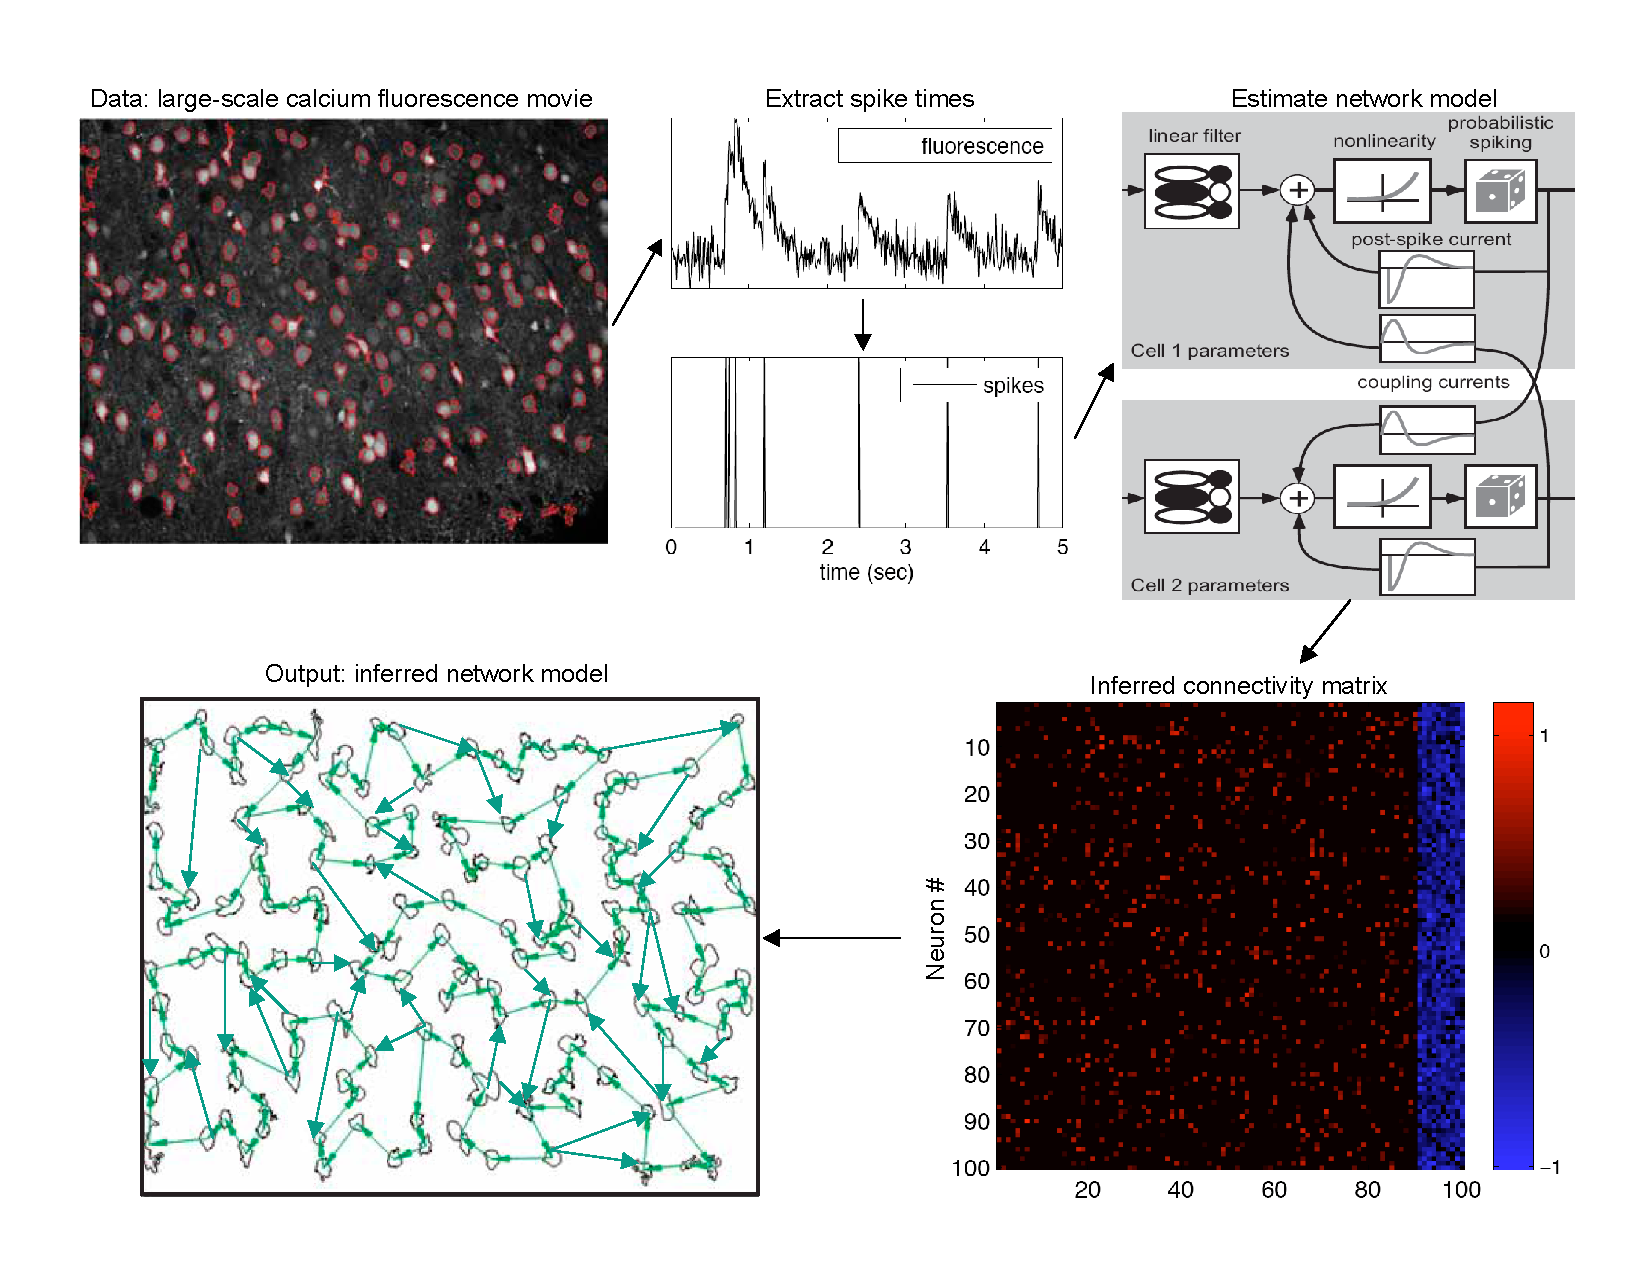
\includegraphics[width=\hsize]{../figs/yuri-paper-schematic} 
	\caption{Schematic overview. The raw observed data is a large-scale calcium fluorescence movie, which is pre-processed to correct for movement artifacts (in the in vivo setting) and find regions-of-interest (i.e., putative neurons); note that we have omitted details of these important preprocessing steps in this paper. Given the fluorescence traces from each neuron, we estimate the underlying spike trains (i.e., in time series of neural activity) using statistical deconvolution methods. Then we estimate the parameters of a network model, given the observed data. Our major goal is to obtain an accurate estimate of the network connectivity matrix, which summarizes the information we are able to infer about the local neuronal microcircuit. This figure adapted from personal communications with R.\ Yuste, B.\ Watson, and A.\ Packer.} 
	\label{fig:data_schematic} 
\end{figure}

\subsection{Simulating a neural population} \label{sec:results:simulations}

To test the described method for inferring functional connectivity from calcium imaging data, we simulated networks (according to our model, Eqs.~\eqref{eqn:glm:definition} -- \eqref{eqn:F:definition}) of spontaneously firing randomly connected neurons. Although simulations ran at $1$ msec time discretization, imaging rate was assumed to be much slower: $5$--$200$ Hz. Simulations lasted anywhere between 5 minutes and 1 hours (of simulated time). 

Model parameters were chosen based on experimental data available in the literature for cortical neural networks \cite{Braitenberg1998,Urquijo2000,Lefort2009,Sayer1990}. More specifically, the network contained 80\% of excitatory and 20\% inhibitory neurons \cite{Braitenberg1998,Urquijo2000}, each respecting Dale's law. Neurons were randomly connected to each other with probability $0.1$ \cite{Braitenberg1998,Lefort2009}. Synaptic weights for excitatory connections, as defined by EPSP peak amplitude, were randomly drawn from exponential distribution with the mean of $0.5 \mu V$ \cite{Lefort2009,Sayer1990}. Inhibitory connections were also drawn from exponential distribution; their strengths chosen so as to balance excitatory and inhibitory currents in the network, and achieve an average firing rate of $\approx 5 $ Hz \cite{Abeles91}. Practically, this meant that the mean strength of inhibitory connections was about 10 times larger than that of the excitatory connections. PSP shapes were modeled as an alpha function \cite{Koch99}, by differencing two exponentials, corresponding to a sharp rise and relatively slow decay \cite{Sayer1990}. We neglected conduction delays, given that the time delay below $\sim 1$ msec expected in local cortical circuit was smaller than the time step of our computer simulation. Each neuron also had an exponential refractory current \cite{Koch99}.

Note that EPSP peak amplitudes cannot be used directly in Eq.~\eqref{eqn:glm:definition}, as a synaptic weight in our model --- $w_{ij}$ in Eq.~\eqref{eqn:glm:definition} --- is a dimensionless quantity representing the change in the spiking probability of neuron $i$ given neuron $j$ fired; whereas EPSP peak amplitude describes physiologically measured change in the membrane voltage of a neuron due to synaptic currents triggered by spike in neuron $j$. We must therefore find a way to relate the two.

Consider the above model for spiking, Eqs.~\eqref{eqn:glm:definition} -- \eqref{eqn:h:definition}.  Let $\delta P$ be the difference between the probability of neuron $i$ spiking given that neuron $j$ spiked in the previous time bin, $P[n_i(t)=1 | n_j(t-\Delta)=1]$, and the probability of neuron $i$ spiking given that neuron $j$ did \emph{not} spike in the previous time bin, $P[n_i(t) | n_j(t-\Delta)=0]$:
\begin{align}\label{eqn:convert:leadin-2}
\delta P &= P[n_i(t)=1 | n_j(t-\Delta)=1] - P[n_i(t)=1 | n_j(t-\Delta)=0] \nonumber
\\ &= \exp[-e^{b_i+w_{ij}\tau_w}\Delta]-\exp[-e^{b_i}\Delta]
\end{align}
\noindent where $\tau_w$ accounts for the decay time constant of the spike history term.   Now consider a simple, stochastic, integrate-and-fire neuron, with baseline voltage zero, spiking threshold one, EPSP amplitude $V_E$, and variance $\sigma_v^2$:
\begin{align}
	V_i(t) &= V_i(t-\Delta) + V_E \delta(n_j(t-\Delta)) + \sigma_v \sqrt{\Delta} \varepsilon_i(t), \qquad &\text{if } V_i(t)<1 \nonumber
\\	V_i(t) &= 0 &\text{if } V_i(t)\geq 1 
\end{align}
In such a model, we again write $\delta P$:
\begin{align}\label{eqn:convert:leadin-3}
\delta P &= \int_1^\infty \mathcal{N}(V_i(t-\Delta),\sigma^2) \text{d}V_i(t-\Delta) - \int_1^\infty \mathcal{N}(V_i(t-\Delta)+V_E,\sigma^2)\text{d}V_i(t-\Delta) \nonumber
\\ &=g(V_E)
\end{align}
A little algebra yields:
\begin{align}
	w_{ij}= \frac{1}{\tau_w}\left(\ln \left[ -\frac{1}{\Delta} \ln \left[g(V_E)+ \exp\left(-\text{e}^{b_i}\Delta\right)\right]\right]-b_i\right)
\end{align}
which we used to obtain $\bw$ from the above mentioned parameters. 
% So, writing $w_{ij}$ as a function of our integrate and fire model, and plugging it back into Eq.~\eqref{eqn:glm:definition}, we say:
% \begin{equation}\label{eqn:convert}
% \w_{ij}\approx\ln(-\ln(e^{-r_i\tau^h}-V_E/V_b)/r_i\tau^h).
% \end{equation}
% \noindent where $r_i=\exp(b_i)$ is the base firing rate of neuron $i$. 


Parameters for the internal calcium dynamics and fluorescence observations were chosen according to our experience with several cells analyzed using algorithm of \cite{Vogelstein2009}, and conformed to previously published results \cite{ImagingManual,HelmchenSakmann96,BrenowitzRegehr07}. %Each parameter was generated from a normal distribution with specified mean and variance at about 30\% of the mean, truncated at the lower bound at about 30\% of the mean value.  
Table \ref{table:caparm} summarizes the details for each of the parameters in our model.

\begin{table}[h!b!p!]
\caption{Table of simulation parameters. $\mathcal{E}(\lambda)$ indicates an exponential distribution with mean $\lambda$, and $\mathcal{N}_p(\mu,\sigma^2)$ indicates a normal distribution with mean $\mu$ and variance $\sigma^2$, truncated at lower bound $p\mu$.  Units (when applicable) are given with respect to mean values (i.e., units are squared for variance).}\label{table:caparm}

\begin{tabular}{lll}
\hline
Total neurons & 10-500 & \# \\
Excitatory neurons & $80$ & $\%$ \\
Connections sparseness & $10$   & $\%$ \\
Baseline firing rate & $5$ & Hz\\
\hline
EPSP peak height 	& $\sim \mathcal{E}(0.5)$ & $\mu$V \\
IPSP peak height 	& $\sim -\mathcal{E}(2.3)$ & $\mu$V \\
EPSP rise time 		& 1 & msec \\
IPSP rise time 		& 1 & msec \\
EPSP decay time 	& $\sim \mathcal{N}_{0.5}(10,2.5)$ & msec \\
IPSP decay time 	& $\sim \mathcal{N}_{0.5}(20,5)$ & msec\\
refractory time 	& $\sim \mathcal{N}_{0.5}(10,2.5$ & msec \\
\hline
Calcium std. $\sigma_c$ & $\sim \mathcal{N}_{0.4}(28,10)$ & $\mu$M\\
Calcium jump after spike, $A_c$ &  $\sim \mathcal{N}_{0.4}(80,20)$ & $\mu$M\\
Calcium baseline, $C_b$ & $\sim \mathcal{N}_{0.4}(24,8)$ & $\mu$M\\
Calcium decay time, $\tau_c$ & $\sim \mathcal{N}_{0.4}(200,60)$ & msec\\
Dissociation constant, $K_d$ & $200$ & $\mu$M \\
\hline
Mean photon budget, $\alpha$ & $1$--$80$ & Kph \\
Baseline fluorescence, $\beta$ & $XXX$ & XXX \\
Signal-dependent noise, $\gamma$ & $XXX$ & XXX \\
Signal-independent noise, $\sigma^F$ & $XXX$ & XXX \\
\end{tabular}
\end{table}


\section{Results}
\label{sec:results}
\subsection{Inferring functional connectivity from simulated calcium imaging data} \label{sec:results:inference}

With neural population activity simulated as described in the previous section, we used our inference algorithms to reconstruct the functional connectivity matrix from simulated fluorescence data. Specifically, we estimated the connectivity matrix using both the embedded-chain-within-blockwise-Gibbs approach as well as factorized approximation. Figure \ref{fig:scatters} shows that factorized approximation was able to provide reconstructions almost as accurately as the exact embedded-chain-within-blockwise-Gibbs approach, $r^2=0.47$ versus $r^2=0.48$, when parameters corresponded to a realistic experiment, given $10$ minutes of simulation data, and a population of $N=25$ neurons. We also estimated the weights using the true spike trains, $r^2=0.7$ (not shown), and the spike trains down-sampled to the frame rates of calcium imaging, $r^2=0.57$. Importantly, the quality of our estimates using the fluorescence traces alone (and no electrophysiological data) approached that using the true down-sampled spike trains.  

%was worse than those obtained from the the true down-sampled spike trainsm although for SNR of fluorescence data the $r^2$ values for obtained reconstructions approached that of down-sampled true spike trains, Figure \ref{fig:recvar-SNR}. Example of what we understand by high SNR (can be used for functional connectivity inference) and low SNR (cannot be used for functional connectivity inference) are shown in Figure \ref{fig:recvar-SNR} on two fluorescence traces from real in-vivo data.
%
%Fluorescence data is generally acquired at low frame rate and, so, one of its main limitations is bad time-resolution of the observed spike trains. To determine the impact of this constraint on the connectivity reconstructions, and, thus, to determine how close calcium imaging may approach reconstructions from spike trains directly observed under comparable conditions, we conducted this experiment. We observed that at intermediate SNR reconstructions from calcium imaging closely resemble(0d such obtained directly from spike trains, and at higher SNR reconstruction with the quality same with original spike trains was achieved, Figure \ref{fig:scatters} and \ref{fig:recvar-SNR}.
%
%\begin{align}
% \label{eqn:likelihoodGLMmoda}
% &E[\ln P[n_i(t)| \bh(t); b_i, k_i, \bw_i, S^{ext}(t)]
% 	=\sum_t \left( n_i(t) \ln J_i(t) - (1-n_i(t)) \exp(J_i(t)) \Delta \right), \\
% \label{eqn:likelihoodGLMmodb}&J_i(t)=b_i+\sum\limits_j \sum\limits_{t'<t} \w_{ij}(t-t')n_{j}(t')=
% b_i+\sum\limits_j w_{ij} h_j(t).
% \end{align}
%
%The sum in Eqs.~\eqref{eqn:likelihoodGLMmoda} and \eqref{eqn:likelihoodGLMmodb} was over the sample of $\{n_i(t)\}_{i\leq N}$, produced with our spike sampling algorithm, discretized over the time-bins $t'$ with the width corresponding to the calcium imaging frame rate (i.e. 30 ms for 33 Hz and 15 ms for 66 Hz). In one of the two cases we considered, EPSP time-profiles were assumed to be ``known'' exponential, and the weights were estimated using reduced histories $h_{i}(t)=\sum_{t'<t} \exp(-(t-t')/\tau^h)n_{i}(t')$ with the time constant $\tau^h=10$ ms (i.e. second equation in Eq.~\eqref{eqn:likelihoodGLMmodb}). In the second case we considered, the time dependence of $\w_{ij}(t)$ was assumed to be unknown and the first equation in Eq.~\eqref{eqn:likelihoodGLMmodb}) was used to correlate $n_i(t)$ with $n_j(t')$ for $t'<t$ up to a given depth $m$.  In this latter case, since each next term in Eq.~\eqref{eqn:likelihoodGLMmodb}) was significantly smaller than the previous one, we found that the best results were obtained if we took $m=1$ (i.e. minimizing number of unknown variables given certain amount of data). In either case, we described the connection weight between two neurons by a scalar quantity $w_{ij}^s=\text{sign}(\w_{ij})\max_{t} |\w_{ij}(t)|$, which thereafter was used to compare true and reconstructed connectivity weights in all examples below.

\begin{figure}[h]
\centering
\begin{minipage}[c]{0.45\hsize}
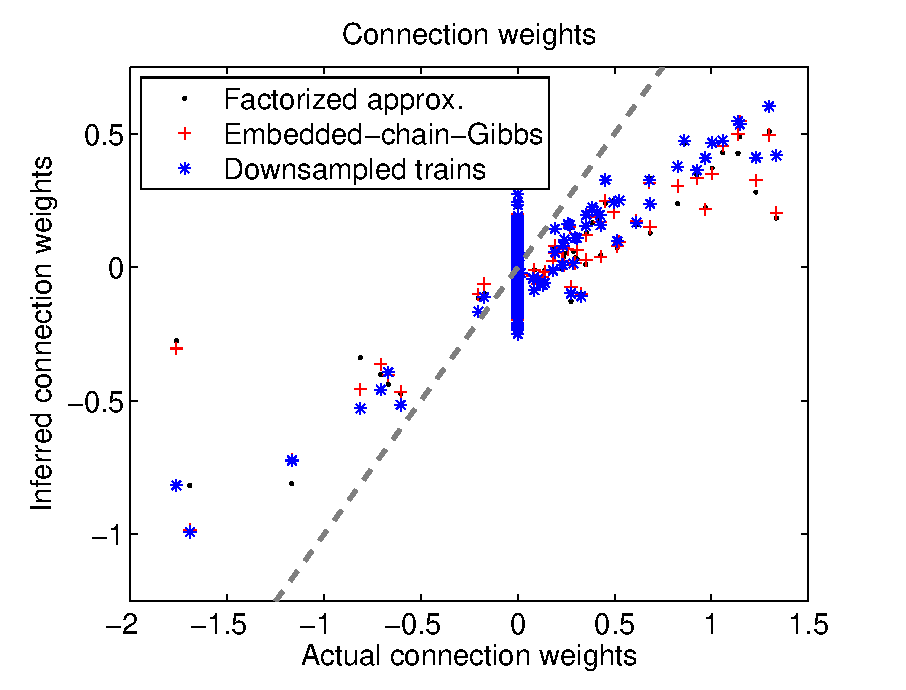
\includegraphics[width=\hsize]{../figs/FigureA3_scatter_three}
\end{minipage}
\begin{minipage}[c]{0.45\hsize}
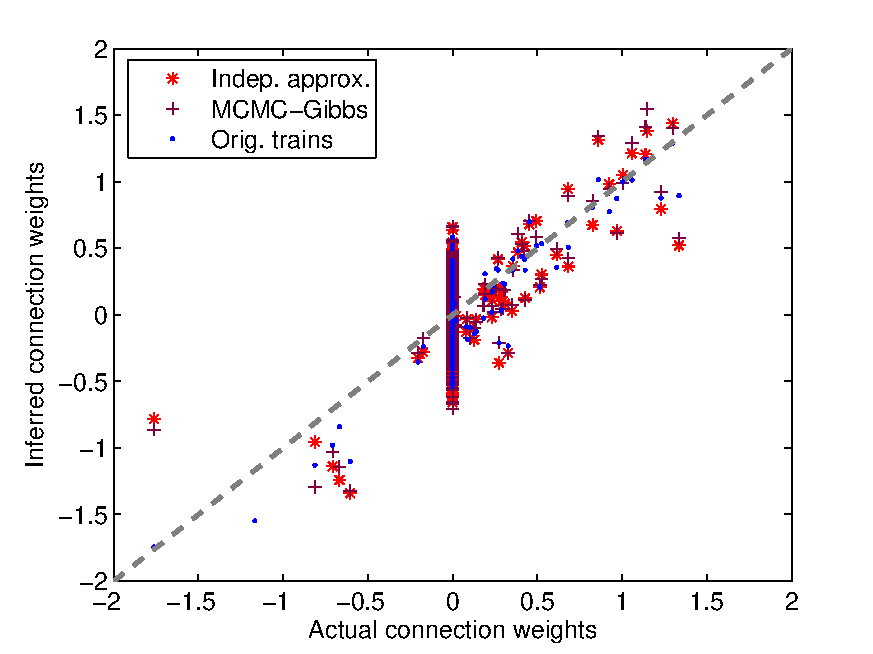
\includegraphics[width=\hsize]{../figs/FigureA3_scatter_three_corrected}
\end{minipage}
\caption{Functional connectivity matrix can be reconstructed from calcium imaging data. Inferred connection weights are shown in a scatter plot versus real connection weights, with inference performed using factorized approximation, exact embedded-chain-within-blockwise-Gibbs approach, and spike trains down-sampled to the frame rate of the calcium imaging. A network of $N=25$ neurons was used, firing at $\approx 5$ Hz, and imaged for 10 min at intermediate SNR (photon budget 10 Kph/neuron/frame; see below). The factorized approximation had an $r^2=0.47$, as compared with the embedded-chain-within-blockwise-Gibbs method's $r^2=0.48$, and $r^2=0.57$ for down-sampled spike trains. The inferred connectivity show a clear scale error (left panel), which we correct using our theoretical scale correction factor (right panel; see Section \ref{sec:scale} for details).} \label{fig:scatters} \end{figure}

\subsection{Impact of coarse time discretization of calcium imaging data and scale factor of inferred connection weights} \label{sec:scale}

As suggested by Figure \ref{fig:scatters}, upon inferring connection weights using down-sampled spike trains (or noisy versions thereof), a scale error is introduced. This is curious because our model was designed to be asymptotically unbiased \cite{PAN03d}. Possible causes of this scale error include (i) insufficient data,  (ii) model misspecification (the simulated model did not conform exactly to our assumed model, due to the shape of PSPs; see Methods for details), or (iii) coarse time discretization.  To investigate what extent of the scale error is caused by the coarse time discretization, we performed the following heuristic argument.

The sufficient statistic for estimating the weights to neuron $i$ in our model is simply $E[X_i(t), \bX (t-\Delta)| \bF; \bth]$, which depends only on $t$ and $t-\Delta$.  If, however, spike trains are down-sampled, such that observations are made only several time-bins, this statistic is not available.  More specifically, it becomes unclear whether certain presynaptic spikes occurred in $t$ or $t-\Delta$.  Thus, some fraction of spikes causally involved in postsynpatic firing will appear coincidental.  The faction of spike that appear coincidental, but are actually causal, corresponds to the expected scale error.

To formalize the above argument, consider the following significantly simplified case of two neurons coupled with a small weight $w_{ij}$, simulated with a time step size of $\Delta$. The sufficient statistic for estimating $w_{ij}$ is simply the expected value of a spike from neuron $i$ at time $t$, given a spike from neuron $j$ at $t-\Delta$:
\begin{align} %\label{eqn:scale:leadin-1}
SS&=E\left[n_i(t) | n_j(t-\Delta)=1\right] %\nonumber \\
=E\left[1-\exp\left(-\text{e}^{b_i+w_{ij}h_{ij}(t)}\right)\right]  \nonumber \\
&\approx \exp(-b_i) \Delta + f'(b_i) \exp(-t/\tau_h) %\nonumber \\
\approx  \exp(-b_i) \Delta + f'(b_i) w_{ij}\tau_h, \label{eqn:SS}
\end{align}
where $f'(b)=df/dXXX$, and $b_i \gg w_{ij}$. The above approximations follow due to XXX, and are required because the expected value is analytically intractable due to the $h_{ij}(t)$ term. 
% where 
% \begin{align}
% \tilde{h}_{ij}^k(t)=\left((1-\Delta \tau^h)h_{ij}(t-\Delta)+1\right)^k
% \end{align}

Now, if the spike trains were down-sampled by a factor $d$, we must further approximate the sufficient statistics. In particular, we would not know precisely in which time of $d$ time-bins the spike from neuron $j$ occurred.  Thus, the best we could do would be:
\begin{align} %\label{eqn:scale:leadin-1}
SS_d=&\sum_{k=1}^{d} E\left[n_i(t) | n_j(t-k\Delta)=1, \{n_j(t-k'\Delta)\}_{k' \neq k}=0\right] %\nonumber \\ &
=\sum_{k=1}^d E\left[1-\exp\left(-\text{e}^{b_i+w_{ij}\tilde{h}_{ij}^k(t)}\right) \right] \nonumber \\
&\approx \exp(-b_i) d\Delta + f'(b) \int\limits_0^\Delta \frac{\text{dt}'}{\Delta} \int\limits_{\Delta}^{\Delta + \mathcal{T}} \text{dt} w_{ij}\exp(-(t-t')/\tau^h) \nonumber \\&
\approx \exp(-b_i) d\Delta +  f'(b)w_{ij}\frac{1-\exp(-\Delta/\tau_h)}{\Delta/\tau_h^2}, \label{eqn:SS_d}
\end{align}
\noindent where $\tilde{h}_{ij}^k(t)$ is the expectation of $h_{ij}(t)$ given a spike from neuron $j$ at $k$ time-bins ago, the approximation follows using the same reasoning as above. The scale error that we expect to obtain from this coarse time discretization is thus: 

\begin{align} \label{eqn:bias}
	\tilde w_{ij} \approx w_{ij} \times\text{scale factor} = w_{ij}  \frac{SS}{SS_d} = w_{ij} \frac{1-\exp(-\Delta/\tau_h)}{\Delta/\tau^h}.
\end{align}

% Unfortunately, we cannot evaluate either $SS$ or $SS_d$ exactly, due to the exponential in $\tilde{h}_{ij}^k(t)$.  Assuming that $\tau^h \ll K \ll 1/r$, we can, however, approximate both by XXX:
% \begin{align}
% 	% SS \approx & r \mathcal{T} + f'(b) \sum_{k=1}^K w_{ij} \exp(-t/\tau^h) \nonumber \\
% 	% 	\approx & r \mathcal{T} + f'(b) w_{ij}\tau^h, \label{eqn:SS}\\
% 	SS_d  	\approx& r \mathcal{T} + f'(b) \int\limits_0^\Delta \frac{\text{dt}'}{\Delta} \int\limits_{\Delta}^{\Delta + \mathcal{T}} \text{dt} w_{ij}\exp(-(t-t')/\tau^h) \nonumber \\
% 		\approx & r \mathcal{T} +  f'(b)w_{ij}\frac{1-\exp(-\Delta/\tau^h)}{\Delta/(\tau^h)^2}. \label{eqn:SS_d}
% \end{align}
% Solving for $w_{ij}$ in terms of $SS$ and $SS_d$, and plugging the resulting values into Eq.~\ref{eqn:scale} yields:
% \begin{equation}\label{eqn:bias}
% w_{ij}\approx \frac{1-\exp(-\Delta/\tau^h)}{\Delta/\tau^h} w_{ij}.
% \end{equation}

% \begin{equation}
% E[n_i(t), n_j(t+\Delta_s) | F_i,F_j] \approx E[n_i(t), n_j(t+\Delta_o) | F_i,F_j]
% \end{equation}
% Our task here is to evaluate the scale error introduced by this approximation, and derive an analytical correction factor.  Let ``causal'' spike-pairs indicate spike-pairs when neuron $j$ spikes in a time bin \emph{preceding} the spike in neuron $i$.  Similarly, Let ``coincident'' spike-pairs indicate those spike-pairs for which both neurons spike within the same time bin.  The coarse time discretization implies that some fraction of causal spike-pairs will appear as coincident spike-pairs.  Thus, we anticipate that the scale error, $\xi$, will be proportional to:
% \begin{equation}
% \xi = \frac{E[\text{number of causal spike-pairs appearing as coincident spike-pairs}]}{E[\text{total number of causal spike-pairs}]}
% \end{equation}
% %Let $n_{ij}$ correspond to the total number of spike-pairs.  
% From Eq.~\eqref{eqn:glm:definition}, we have the probability of a spike from neuron $i$ in time bin $t$, given a spike from neuron $j$ in some previous time bin, $\mathcal{T}$:
% \begin{align}
% E[n_i(t) | n_j(t-\mathcal{T})] 
% &\approx 1-\exp(-\text{e}^{b + w_{ij} E[h_{ij}(t) | n_j(t-\mathcal{T})=1]} \Delta) 
% \end{align}
% where we define the expected spike history input conditioned on a spike from neuron $j$ at time $\mathcal{T}$:
% \begin{align}
% E[h_{ij}(t) | n_j(t-\mathcal{T})] &= \left((1-\Delta_s/\tau^h) E[h_{ij}(t-\Delta_s)] + 1\right)^{\mathcal{T}/\Delta_s}
% % = \sum_t n_i(t) P[n_i(t) | n_j(t-\mathcal{T})]  
% % = \sum_t  1-\exp(-\text{e}^{b + w_{ij} h_{ij}(t)} \Delta)
% %\exp{-t/\tau^h}
% %\approx r \mathcal{T} + f'(b) \int^{\mathcal{T}}_0  w_{ij} \exp(-t/
% %\tau^h) dt = XXX
% \end{align} 
% When we use a coarse time discretization, Eq.~\eqref{eqn:E[h]} changes by replacing each $\Delta_s$ by a $\Delta_o$.  
% 
% this above expectation changes to:
% \begin{align}
% E[h_{ij}(t) | n_j(t-\mathcal{T})] &= \left((1-\Delta_o/\tau^h) E[h_{ij}(t-\Delta_s)] + 1\right)^{\mathcal{T}/\Delta_s}
% \end{align} 
% 
% Similarly, we can compute the number of causal spike-pairs that appear as coincident spike-pairs, given our coarse time discretization:
% 
% % In order to estimate $w_{ij}$, therefore, we need to empirically observe the number of spike-pairs such that the first neuron fired after the second neuron over some small period of time $\tau^h \ll \mathcal{T} \ll 1/r$. 
% % 
% % With this count, we empirically estimate the spike-triggered spiking probability of the first neuron, conditioned on the firing of the second neuron, and subsequently estimate the connection weight $w_{ij}$. Per time period $\mathcal{T}\ll 1/r$, the average number of such spike-pairs corresponding to connection weight $w_{ij}$ is:
% % \begin{equation}\label{eqn:scale:leadin-1}
% % n_{12} \approx r \mathcal{T} + f'(b) \int^{\mathcal{T}}  w_{ij} \exp(-t/\tau^h) dt.
% % \end{equation}
% % 
% % Now, assume that observed spike trains were additionally down-sampled into time-bins of size $\Delta$. We now only count the spike-pairs such that the spike of the first neuron and the second neuron occurred in different time-bins of size $\Delta$. Per time period $\mathcal{T}$, the average number of such spike-pairs in down-sampled spike trains can be calculated as follows. We consider all spike-pairs such that the spike of the second neuron occurred in one time bin, $t'\in [0,\Delta]$, and the spike of the first neuron occurred in any of the strictly subsequent time bins up to $\mathcal{T}$, $t\in [\Delta,\mathcal{T}]$. Taking into account that position of the first spike, $t'$, is uniformly distributed in $[0,\Delta]$, the average number of such spikes of the first neuron per spike of the second neuron, observed empirically, is:
% \begin{equation}\label{eqn:scale:leadin-2}
% n^{\Delta_o}_{12} \approx r \mathcal{T} + f'(b) \int\limits_0^\Delta \frac{\text{dt}'}{\Delta} \int\limits_{\Delta}^{\mathcal{T}} \text{dt} \exp(-(t-t')/\tau^h)
% = r \mathcal{T} +  f'(b)\frac{1-\exp(-\Delta/\tau^h)}{\Delta/{\tau^h}^2}.
% \end{equation}
% Plugging these results into Eq.~\eqref{eqn:bias_correction_factor}, we obtain:
% %\comment{If we were to naively apply GLM Eq.~\eqref{eqn:scale:leadin-1} in this latter case, we would have underestimated $w_{ij}$ by a factor $\approx (n^{\Delta_o}_{12}-r \mathcal{T})/ (n_{12}-r \mathcal{T})$, corresponding to smaller spike-triggered probability observed empirically in down-sampled spike-trains. This ratio is the scaling factor that we observe:}
% \begin{equation}\label{eqn:bias}
% \xi=\frac{n^{\Delta_o}_{12}-r \mathcal{T}}{n_{12}-r \mathcal{T}}\approx \frac{1-\exp(-\Delta/\tau^h)}{\Delta/\tau^h}.
% \end{equation}
% %\comment{In Figure \ref{fig:bias} we plotted Eq.~\eqref{eqn:bias} versus scale factor empirically observed from our simulations for different values of $\Delta$. As can be seen from}
% Figure \ref{fig:bias} shows that this theoretical approximation corresponds well to our empirically measured scale factor.

%% Spike trains, necessary to evaluate functional connectivity matrix $\bw$, here were inferred with discretization into time-bins corresponding to the frame-rate of calcium imaging fluorescence data. In principle, one could use super-resolution feature of \cite{Vogelstein2009} to obtain spike trains with arbitrarily small time step $\Delta\rightarrow 0$. However, the problem in that case is that the spikes, inferred from fluorescence data, contain inaccuracy in their temporal position $\approx 1/$frame-rate,  due to the time-discretization of the underlying fluorescence trace.Thus, when we super-resolve spikes using \cite{Vogelstein2009}, the spike pairs such that a spike of neuron $i$ closely follows a spike of neuron $j$ can be often confused with such where a spike of neuron $j$ closely follows a spike of neuron $i$. It, therefore, becomes impossible to determine which neuron fired first, and which neuron was pre-synaptic or post-synaptic in given pair of neurons $i$, $j$. More specifically,
%%because we rely on empirically counting close spike pairs in a set of spike trains to estimate the spike-triggered probabilities for spikes of different pairs of neurons, $i$ and $j$, which then allow estimating $w_{ij}$, above disordering of close spike pairs results in dramatic noise component in our estimate for the functional connectivity matrix by not allowing to effectively distinguish $w_{ij}$ and $w_{ji}$.
%when using $\Delta \rightarrow 0$, we observed large errors in $\bw$, $var[\bw] \propto \bw + \bw^T$ - because of inaccuracies in temporal position of spikesinferred from calcium imaging it became impossible to reliably distinguish which neuron causally preceded which other neuron, and only a-causal connectivity matrix $(\bw + \bw^T)/2$ could be determined.

% To circumvent this problem, we (down-)sampled the time-axis in bins of size $\Delta=1/$frame-rate, and treated all spike pairs that occurred within the same time-bin as coincidental. This successfully counteracted the above problem and, additionally, allowed to perform calculations substantially faster by using larger $\Delta$. At the same time, this resulted in scale bias that all our inferred  connectivity matrices consistently exhibited, Figure \ref{fig:scatters}. This bias may be successfully understood and corrected from the following time-discretization argument. Specifically, estimating the magnitude of the connection weight $w_{ij}$ is based on empirically evaluating the spike-triggered probability of neuron $i$ to fire, conditioned on neuron $j$. Most significant change in the spiking probability of neuron $i$, conditioned on neuron $j$, occurs within $\tau^h \approx 10-20$ msec from a spike of neuron $j$. When spike trains are down-sampled into large time-bins, e.g. $\Delta = 30$ msec, a significant fraction of close spike pairs appears coincident and not causal, as both spikes from neuron $i$ and neuron $j$ within $\approx \tau^h$ from each other are often assigned to the same time-bin. As we discussed in the previous paragraphs, such close spike pairs typically introduce a great deal of noise in the estimate of $\bw$. When $\Delta$ is large, however, most of such unreliable spike pairs would be considered coincidental and would not affect $\bw$ estimate. At the same time, all of such close pairs would be lost if we were to empirically evaluate the spike-triggered probabilities, which would have led us to believe in a lower than the actual  $w_{ij}$.
This is the scale bias that we observe. In Figure \ref{fig:bias} we plot the scale bias from Eq.~\ref{eqn:bias} versus that empirically deduced from our simulations for different values of $\Delta$. As can be seen in Figure \ref{fig:bias}, Eq. \ref{eqn:bias} describes observed scale bias very well.
	
An alternate way of dealing with this scale error would be to sub-sample spike trains, as discussed in \cite{Vogelstein2009}, to obtain spike train inferences at the desired temporal resolution.  This possibility was not pursued here, as this approximation was sufficient for this work.

\begin{figure}[h]
\centering
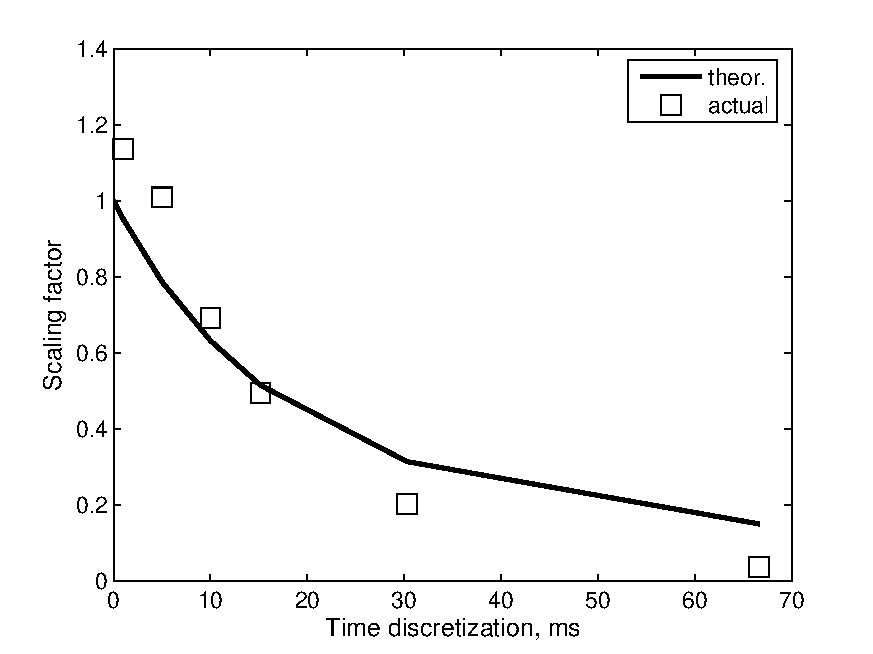
\includegraphics[width=3in]{../figs/FigureA4_scale_bias}
\caption{The low-frame rate of calcium imaging can explain the scale factor in inferred connectivity weights in Figure \ref{fig:scatters}.  Theoretically, scale factor may be evaluated by calculating what fraction of spikes from two neurons would occur within a single time-bin of width $\Delta$ (c.f. Eq.~\eqref{eqn:bias}).  
Plotted such theoretically calculated scale factor (line) vs. that observed empirically from our simulations (box), from a simulation of $N=25$ neurons, $T=10$ min. The error-bars correspond to 95\% confidence intervals for scale factor estimate.}
\label{fig:bias}
\end{figure}

\subsection{Impact of using priors on the inference}

Taking into account simple prior information about the connectivity matrix results in dramatic improvement of the inferred connectivity matrix using the same data.%; facilitating successful reconstruction from as little as $5$ min of calcium imaging data, and for $T\approx 10$ min achieving the same level of accuracy otherwise requiring up to $T\approx 1$ hour of calcium imaging, Figure \ref{fig:recvar-NT}. 
For example, imposing a sparse prior on a simulation of a network of $N=50$ neurons imaged for $T=10$ min, increased $r^2$ from $r^2=0.64$ to $r^2=0.85$ (Figure \ref{fig:sparse}). Furthermore, the weights estimated using the sparse prior more reliably provide true connectivities, as well as the appropriate sign (i.e., exicitatory or inhibitory) of each presynaptic neuron (Figure \ref{fig:distros}). Unfortunately, introducing a sparse prior further scales connectivity estimates, invaliding our analytic scale correction factor.  Thus, a sparse prior can provide a more rapid estimate of relative connection strengths, but not absolute connection strengths, at this time. 

Dale's prior, on the other hand, only leads to $\approx 10\%$ change in $r^2$ of the reconstructed connectivity matrix for this simulation, and was not found significant. Further, imposing Dale's prior when the sparse prior was initially enforced, typically resulted in no improvement to $\bw$ at all (not shown).  As the sparse prior result achieved reconstruction accuracy close to the down-sampled spike train limit, there was limited room for improvement using Dale's prior, and thus, it is not pursued further here.

\begin{figure}[h]
\centering
\begin{minipage}[c]{0.45\hsize}
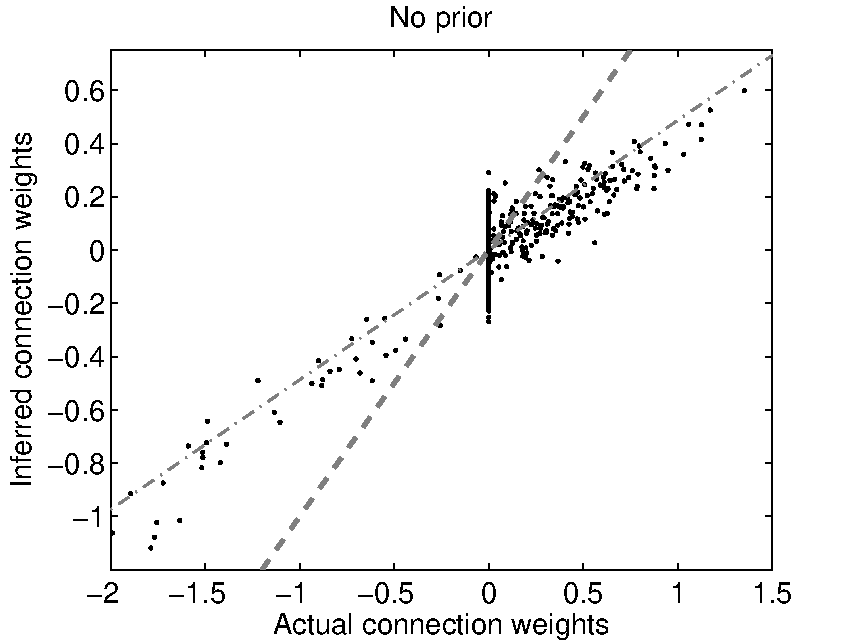
\includegraphics[width=\hsize]{../figs/FigureA10_regular_sol}
\end{minipage}
\begin{minipage}[c]{0.45\hsize}
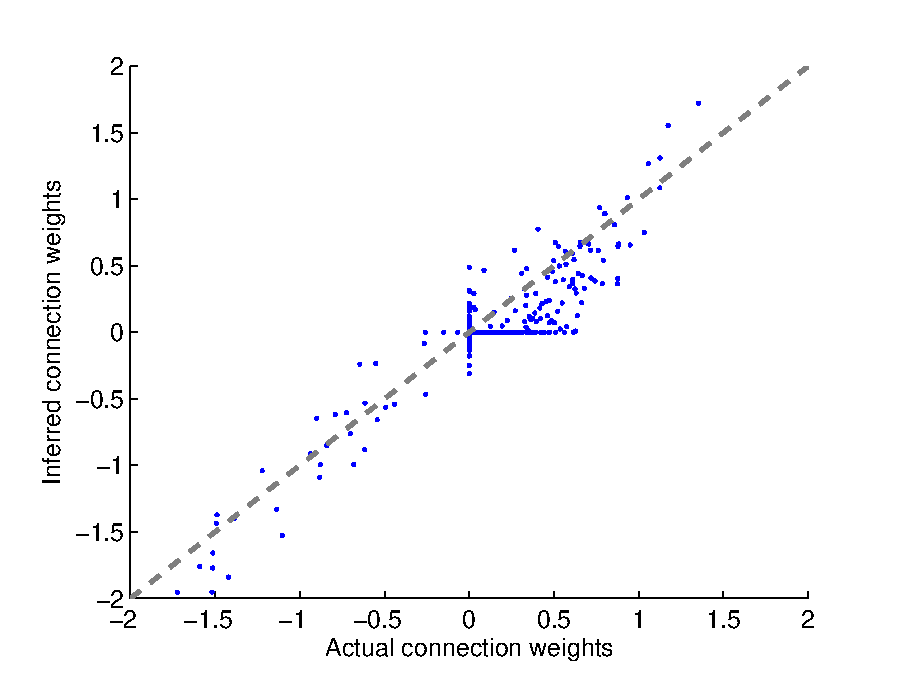
\includegraphics[width=\hsize]{../figs/FigureA10_sparse_sol}
\end{minipage}
\caption{Connection weights reconstructed using no prior ($r^2=0.64$; left panel) and a sparse prior ($r^2=0.85$; right panel) are shown in a scatter plot for a network of $N=50$ neurons, firing at $\approx 5$ Hz, and imaged for $T=10$ min. Clearly, the sparse prior reduces the relative error, as indicated by comparing the relative distance between the data points (black dots) to the best linear fit (black line), across the two panels.  }
\label{fig:sparse}
\end{figure}

\begin{figure}[h]
\centering
\begin{minipage}[c]{0.45\hsize}
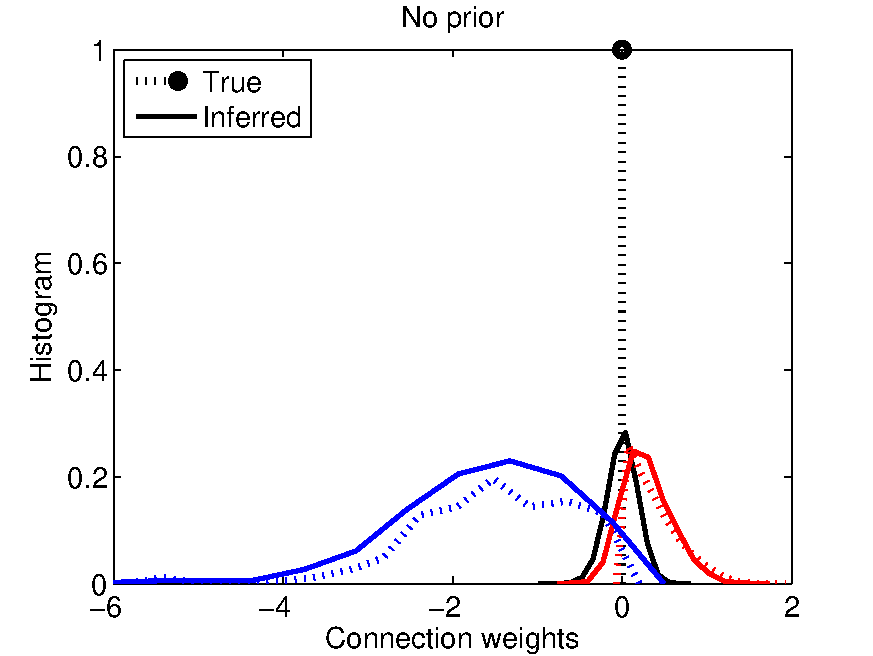
\includegraphics[width=\hsize]{../figs/FigureA3_hist_glm200}
\end{minipage}
\begin{minipage}[c]{0.45\hsize}
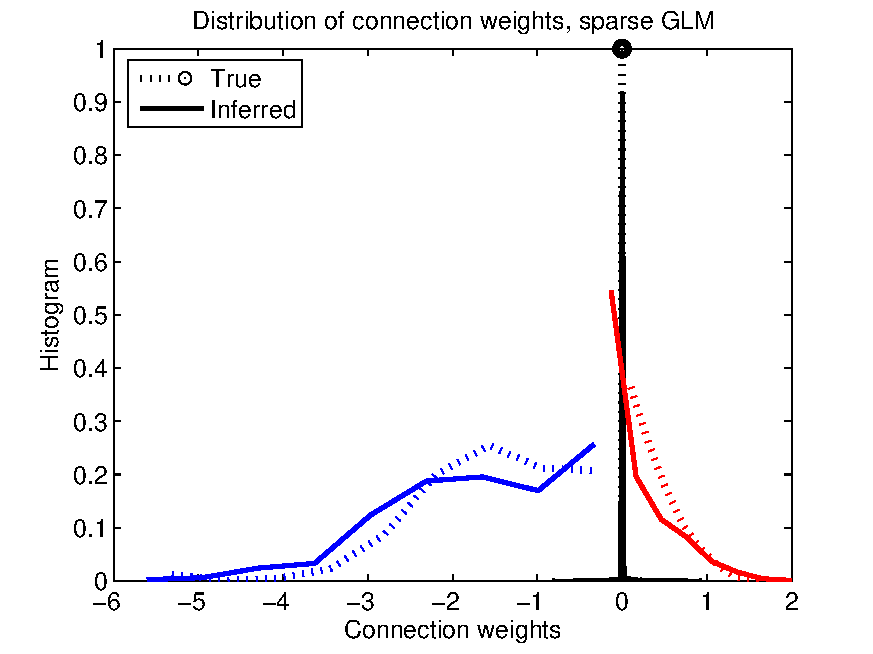
\includegraphics[width=\hsize]{../figs/FigureA3_hist_spa200}
\end{minipage}
\caption{Imposing a sparse prior on the distribution of connectivity weights, facilitates improving the inferred weights given the same amount of data. Shown here is the distribution of inferred connection weights using no prior (left panel) and a sparse prior (right panel) vs. true distributions. When the sparse prior is enforced, the appropriate number of connected pairs is identified (black lines), as well as the correct distribution of excitatory and inhibitory weights (red and blue lines, respectively). Distributions are shown for a network of $N=200$ neurons, firing at $\approx 5$ Hz, and imaged for $T=10$ min.}
\label{fig:distros}
\end{figure}


\subsection{Impact of experimental factors on estimator accuracy}

What minimal conditions for the experimental setup should be met to for sufficient reconstruction accuracy of the connectivity from calcium imaging data? In Figures \ref{fig:recvar}--\ref{fig:recvar-NT} we address this question. Figure \ref{fig:recvar} shows the quality of the inferred connectivity matrix as function of the imaging frame rate --- imaging frame rates $30$--$60$ Hz are needed to achieve meaningful reconstruction results. Frame rates $\approx 100$ Hz allow achieving the same level of the connectivity matrix reconstruction that is possible with the exact knowledge of the true spike trains. Imaging frame $30$--$60$ Hz are already in progress in existing experimental setups \cite{NguyenParker01,ReddySaggau05,Iyer06,SalomeBourdieu06,ReddySaggau08}, each with the ability to significantly increase imaging rate, but costing a reduction in the number of observable neurons.

\begin{figure}[h]
\centering
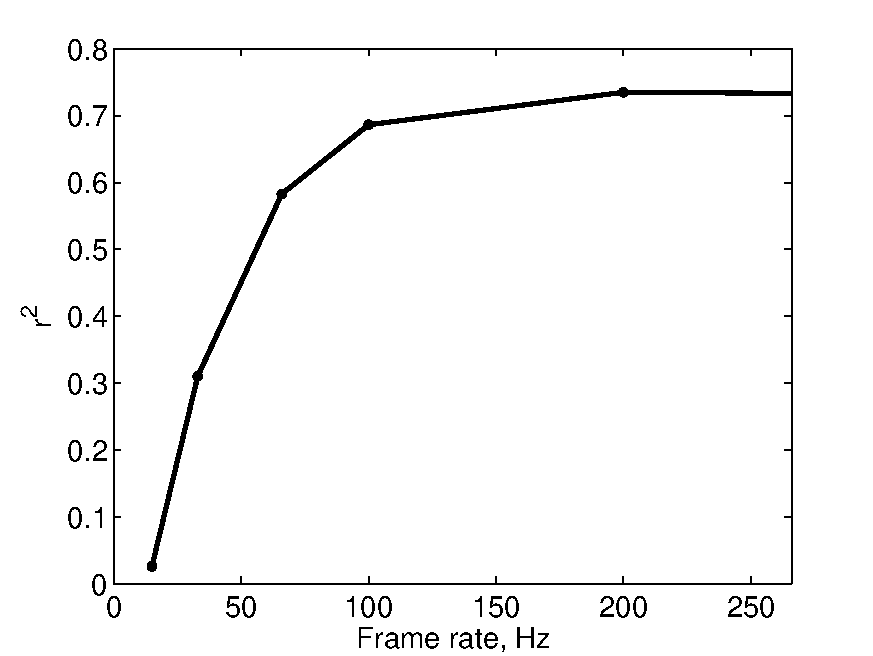
\includegraphics[width=3in]{../figs/FigureA5_recvar}
\caption{Accuracy of the inferred connectivity as function of the frame rate of calcium imaging.  A network of $N=25$ neurons, firing at $\approx 5$ Hz and imaged for $T=10$ min was simulated, and weights were inferred. At $100$ Hz, $r^2$ using calcium imaging data reached the same level of accuracy as using the true spike trains from this simulation, indicating the further improvement could not be achieved by a further increase in frame rate.}
\label{fig:recvar}
\end{figure}

Figure \ref{fig:recvar-SNR} shows the quality of the inferred connectivity matrix as function of effective SNR and photon budget. Operationally, we define effective SNR as
\begin{equation}
\text{eSNR}=\frac{E[F_i(t)-F_i(t-1)|n_i(t)=1]}{E[(F_i(t)-F_i(t-1))^2|n_i(t)=0]^{1/2}},
\end{equation}

\noindent and photon budget as $\gamma^{-1}$.  Photon budget corresponds to the number of photons collected from single neuron within a single frame, at the peak of fluorescence intensity. XXX i don't see how this is true. XXX Note that the relationship between photon budget and eSNR depends on a number of other parameters, $\{\alpha,\beta,\sigma^F, K_d\}$, as well as the calcium concentration (which depends on spike rate, as well as $\{\tau^c, A, C^b\}$). From our experience with the analysis of real cells \cite{Vogelstein2009}, the eSNR for data collected at $15$ Hz was $\approx 3$ for in vitro data sets, and $\approx 9$ for in vivo data sets (c.f. Figure \ref{fig:example_traces}). As can be seen from Figure \ref{fig:recvar-SNR}, the effective SNR necessary for optimal reconstructions given a particular frame rate was $\approx 5$. This eSNR corresponded to photon budgets of $\approx 10$ Kph/neuron/frame. Any lower, and reconstruction accuracy declined rapidly.  

\begin{figure}[h]
\centering
\begin{minipage}[c]{0.6\hsize}
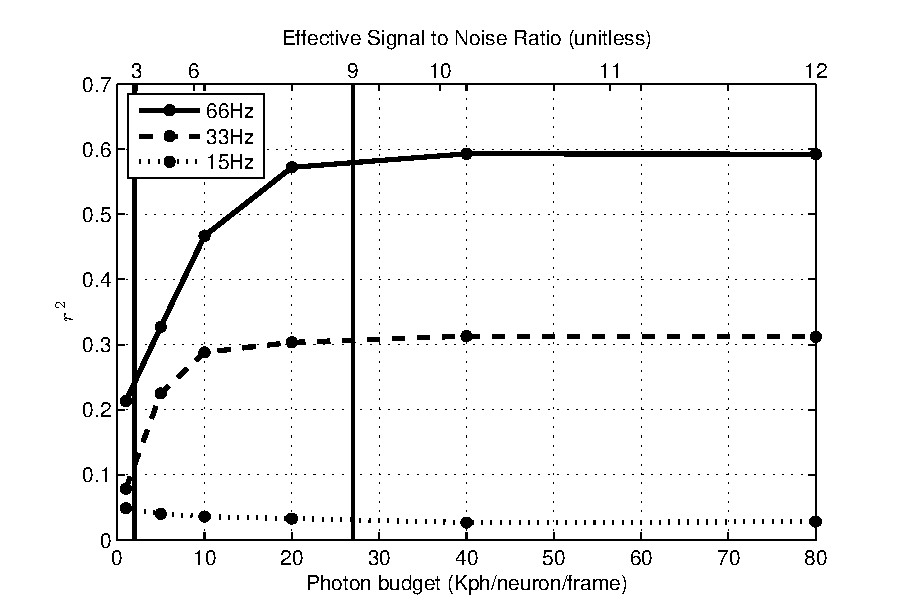
\includegraphics[width=\hsize]{../figs/FigureA6_recvar_SNRb}
\end{minipage}
\caption{Accuracy of inferred connectivity as function of the noise amount in the calcium imaging data, as quantified by (i) eSNR and (ii) thousands of photons, per frame, per neuron (Kph/frame/neuron), for frame rates of 1, 5, 10, 15, 33, and 66 Hz. Photon counts on the order of $10$--$20$ Kph/frame/neuron are required to achieve the upper bound determined by the frame rate. The connectivity matrix here was inferred from simulated fluorescence data using factorized approximation algorithm and the sparse prior. Simulation conditions are the same as in Figure \ref{fig:recvar}.  Vertical black lines correspond to the two example traces in Figure \ref{fig:example_traces}.}
\label{fig:recvar-SNR}
\end{figure}

Finally, Figure \ref{fig:recvar-NT} shows the quality of the inferred connectivity matrix as function of the experiment duration. The minimal amount of data for a particular $r^2$ depended substantially on whether the sparse prior was enforced. In particular, when not imposing a sparse prior, the calcium imaging duration necessary to achieve $r^2=0.5$ for the reconstructed connectivity matrix was $T\approx 10$ min, and $r^2=0.75$ was achieved at $T\approx 30$ min. With a sparse prior, $r^2>0.7$ was achieved already at $T\approx 5$ min. Furthermore, we observed that the accuracy of the reconstruction did not deteriorate with the size of the imaged neural population: the same reconstruction quality was observed with the same amount of data for $N=50$--$200$ neurons.  This, at first unexpected result, is the direct consequence of the structure of the covariance matrix for $\bw$, as will be discussed below. In all cases, good reconstructions were possible with only $T\sim 5$--$30$ min of calcium imaging data.

\begin{figure}[h]
\centering
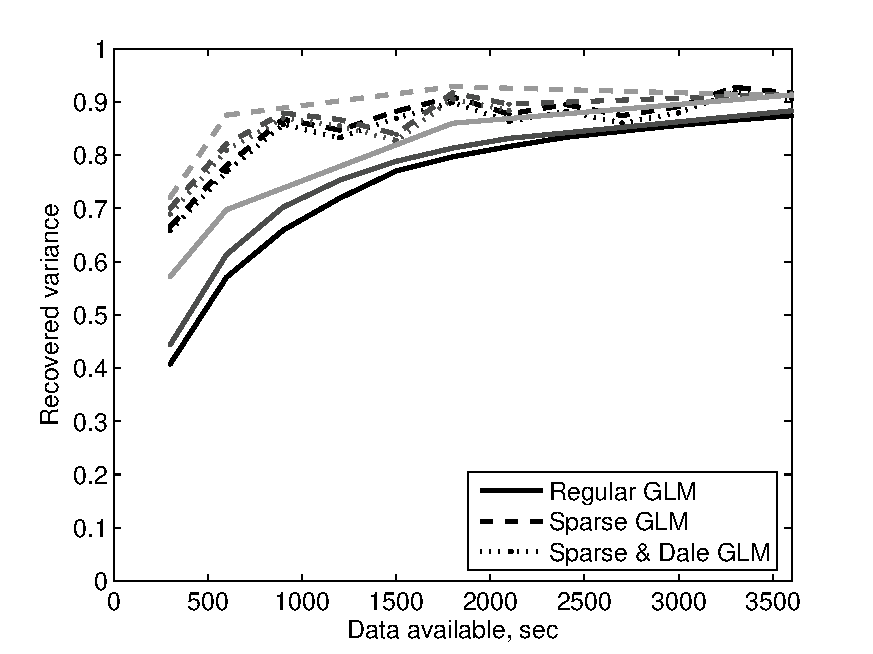
\includegraphics[width=3in]{../figs/FigureA7_recvar_NT}
\caption{Accuracy of inferred connectivity as function of the imaging time and neural population size. Incorporating a sparse prior dramatically increases the reconstruction's quality (dashed lines), over the no prior assumption (solid lines), given the same experimental duration. When the sparse prior is imposed, $T=5$ min is already sufficient to recover $70\%$ of the variance in the connection weights. Incorporating Dale's prior leads to only marginal improvement (dotted line). Furthermore, reconstruction accuracy does not strongly depend on the neural population size, $N$. Here, neural population from $N=10$ to $N=200$ were simulated for different $T$, $N=100$ and $200$ are shown (black and gray, respectively).  Inhibitory weights for networks of different sizes were chosen to ensure mean firing rate $\approx 5$ Hz, although actual firing rate varied somewhat.}
\label{fig:recvar-NT}
\end{figure}

\subsection{Accuracy of the estimates and Fisher information matrix} \label{sec:methods:accuracy_Fisher}

Here we calculate theoretically the amount of spike trains data necessary to accurately estimate the functional connectivity matrix, $\bw$. For clarity, we assume here that $\Delta \rightarrow 0$, and so $f(J)\approx e^J\Delta$, and that the spike trains are known perfectly, i.e. there is no corruption due to inference from low-SNR calcium imaging data (an assumption validated by the above results). We also assume that the spikes only couple over a single time bin, so $h_{ij}(t)\equiv n_j(t-\Delta)$. Then, we can write the likelihood for the weights:
\begin{align}\label{eqn:fisher-glm}
% \begin{array}{rl}
-\ln P[\bw | \bX] &\propto -\ln P[\bX | \bw] =
\sum\limits_{i,t} \left[ n_i(t) \ln f(J_i(t)) + (1-n_i(t)) (1-f(J_i(t))) \right], \\
J_i(t) &= b_i(t) + \sum\limits_j w_{ij} h_{ij}(t) = b_i(t) + \sum\limits_j w_{ij} n_j(t-\Delta) 
%h_{ij}(t) &= n_j(t-\Delta)
.
% \end{array}
\end{align}
The Fisher information matrix for $P[\bw | \bX]$ is therefore:
\begin{multline}\label{eqn:fisher-def}
% \begin{array}{rl}
COV^{-1}_{ij;i'j'}=\left[\frac{\partial (-\ln P[\bw | \bX])}{\partial \w_{ij}\partial \w_{i'j'}}\right]
=\\-\delta_{ii'}\sum\limits_t\left[
n_i(t)n_{j}(t-\Delta)n_{j'}(t-\Delta)\left(-\frac{f'(J_i(t))^2}{f(J_i(t))^2} +
\frac{f''(J_i(t))}{f(J_i(t))}\right) -(1-n_i(t))n_{j}(t-\Delta)n_{j'}(t-\Delta)f''(J_i(t))\right],
% \end{array}
\end{multline}
where $f'$ and $f''$ correspond to the first and the second derivatives of our linking function (c.f Eq.~\eqref{eqn:glm:definition}), and $\delta_{ii'}$ is the Kronecker's delta symbol, i.e., $\delta_{ii'}=1$ for $i=i'$, and $\delta_{ii'}=0$ otherwise.  Letting $f(J)=e^J\Delta$, the first term in the sum in Eq.~\eqref{eqn:fisher-def} cancels out, and the rest may be rewritten as:
\begin{align}\label{eqn:fisher}
% \begin{array}{rl}
COV^{-1}_{ij;i'j'}
&=\delta_{ii'} T P[n_i(t)=0, n_j(t-\Delta)=1, n_{j'}(t-\Delta)=1]% \times \\&
\times E[e^{J_i(t)}|n_i(t)=0, n_j(t-\Delta)=1, n_{j'}(t-\Delta)=1] \nonumber \\
&= \delta_{ii'}T\left[(r \tau^h)\delta_{jj'}+O((r \tau^h)^2)\right]r.
% \end{array}
\end{align}
Here, $TP[n_i(t)=0, n_j(t-\Delta)=1, n_{j'}(t-\Delta)=1]$ describes the number of nonzero
terms in Eq.~\eqref{eqn:fisher-def}, corresponding to the condition that
$(1-n_i(t))n_{j}(t-\Delta)n_{j'}(t-\Delta)$ is only nonzero when 
$n_i(t)=0$, $n_j(t-\Delta)=1$, and $n_{j'}(t-\Delta)=1$.  We let $r=E[e^{J_i(t)}|n_i(t)=0, n_j(t-\Delta)=1, n_{j'}(t-\Delta)=1]$  correspond to the average value of $f''(J_i(t))$, conditional on such nonzero events.  $r\tau_h \ll 1$ is the probability for a neuron to spike over the time-interval $\tau_h$.

The Fisher information matrix is block-diagonal, $COV^{-1}_{ij;i'j'} \propto \delta_{ii'}$, due to the structure of the log-likelihood $P[\bX | \bw]$ (it is a sum over $i$ of independent terms), Eq.~\eqref{eqn:fisher-glm}.From Eq.~\eqref{eqn:fisher}, we observe that Fisher information matrix is predominantly diagonal, because $COV^{-1}_{ij;i'j'} \propto \delta_{ii'}\delta_{jj'}$, and thus the covariance matrix, $COV$, can be computed trivially:
\begin{equation}
COV = (rT)^{-1} (r \tau^h I + O((r \tau_h)^2))^{-1} = (r^2 \tau_h T)^{-1} I + O((r \tau_h)^2),
\end{equation}
\noindent where $I$ is the Identity matrix of appropriate size.  For successful determination of the functional connectivity matrix $\bw$, $COV$ should be made smaller than the typical scale $\langle \bw^2\rangle$, so we require that:
\begin{equation}
T \approx (\langle \bw^2 \rangle r^2  \tau^h)^{-1}.
\end{equation}
For typical values of $\langle\bw^2\rangle\approx 0.1$, $r\approx 5$ Hz and $ \tau_h \approx 10$ msec, this estimate provides $T$ of the order of hundreds of seconds. This theoretical estimate of the necessary amount of fluorescent data is in good agreement with our simulations.

Finally, because $COV^{-1}$ is diagonal, this scale of $COV$ does not depend on the number of neurons in the imaged neural population, $N$. Thus, the variance of the estimate $\bw$ does not degrade with the size of the imaged population, $N$, for the same amount of data, $T$.

\subsection{Impact of strong correlations and deviations from generative model on the inference}

``Anatomical'' connectivity was recovered in our experiments despite potential problems noted in the literature, e.g. such as common input from correlated neurons \cite{Nykamp05,NYK06}, or unobserved neurons \cite{Vidne08}. %This is primarily due to the particular form of the activity in our neural networks, whereas firing of neurons occurred independently, thus, allowing GLM explore the full range of possible input configurations and disentangle common inputs.
Estimation of the functional connectivity is fundamentally rooted in observing changes in the spike rate conditioned on the state of the other neurons. Intuitively, such estimation can be compared to observing changes in $f({\bf n}(t))\propto\exp(\sum_j \w_{ij}n_j(t))$ for different neural configurations ${\bf n}(t)$, i.e. estimating a vector ${\bf w}_i$ from a number of dot-products ${\bf w}_i\cdot {\bf n}(t)$. In order to properly estimate all components of ${\bf w}_i$ the set of available ${\bf n}(t)$ should be rich enough to span all $N$ dimensions of ${\bf w}_i$. In case of independent firing such condition is clearly satisfied.  Should this condition be violated, however, e.g. due to high correlation between spiking of few neurons, spike trains may not provide access to the true vector ${\bf w}_i$, and the connection weights inferred from such activity data may effectively ``aggregate'' true connection weights in arbitrary linear combinations.

We carried out a simulation of hypothetical ``strongly'' coupled neural network, where in addition to weak sparse connectivity we introduced sparse random strong connectivity component. In a sense, we allowed a fraction of neurons to couple strongly to the other neurons, thus, making them ``command'' neurons ``driving'' the activity of the rest of the population. The strength of strong connectivity component was chosen to dynamically build up the actual firing rate from the baseline rate of $r=\exp(b)\approx 1$ Hz to approximately $5$ Hz. Such a network showed patterns of activity very different from the weakly coupled networks inspected above (Figure \ref{fig:rasters}, top right). In particular, a large number of highly correlated events across many neurons were evident in this network. As expected, our algorithm was not able to identify the true connectivity matrix correctly in this scenario (Figure \ref{fig:rasters}, bottom right panel).  For ease of comparison, the left panels show a ``typical'' network (i.e., one lacking many strongly coupled neurons), and its associated connectivity inference.  Note that the observability of the strongly coupled neurons does not save our inference.

\begin{figure}[h]
\centering
\begin{minipage}[c]{0.45\hsize}
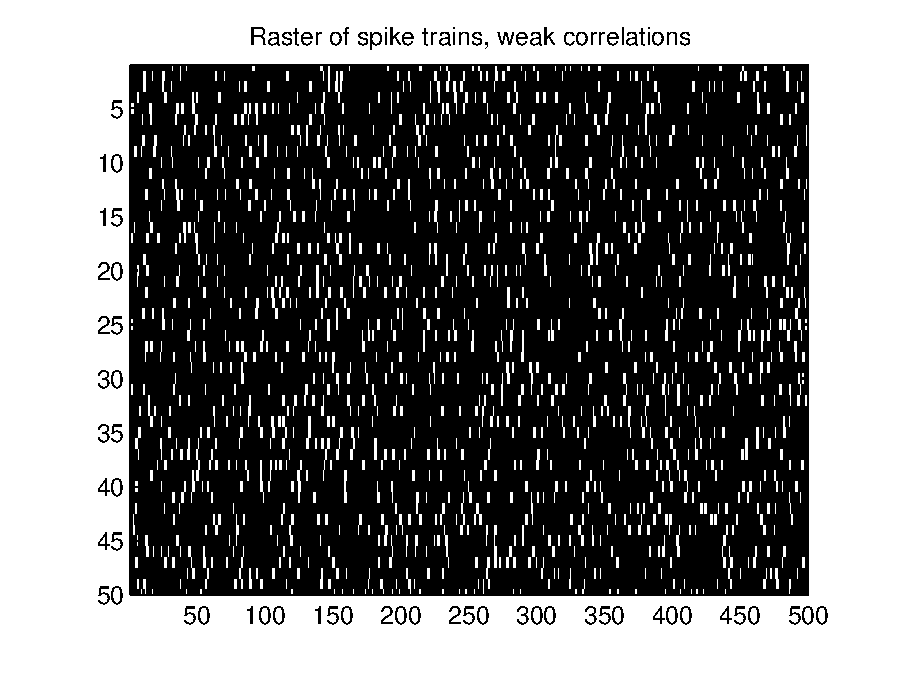
\includegraphics[width=\hsize]{../figs/Figure7b_raster_weak}
\end{minipage}
\begin{minipage}[c]{0.45\hsize}
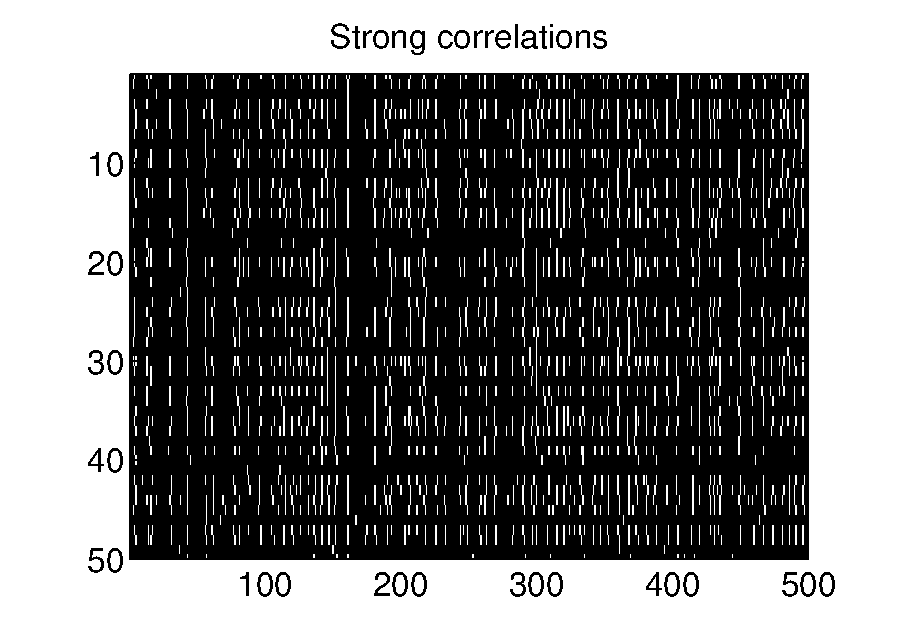
\includegraphics[width=\hsize]{../figs/Figure7a_raster_strong}
\end{minipage}
\begin{minipage}[c]{0.45\hsize}
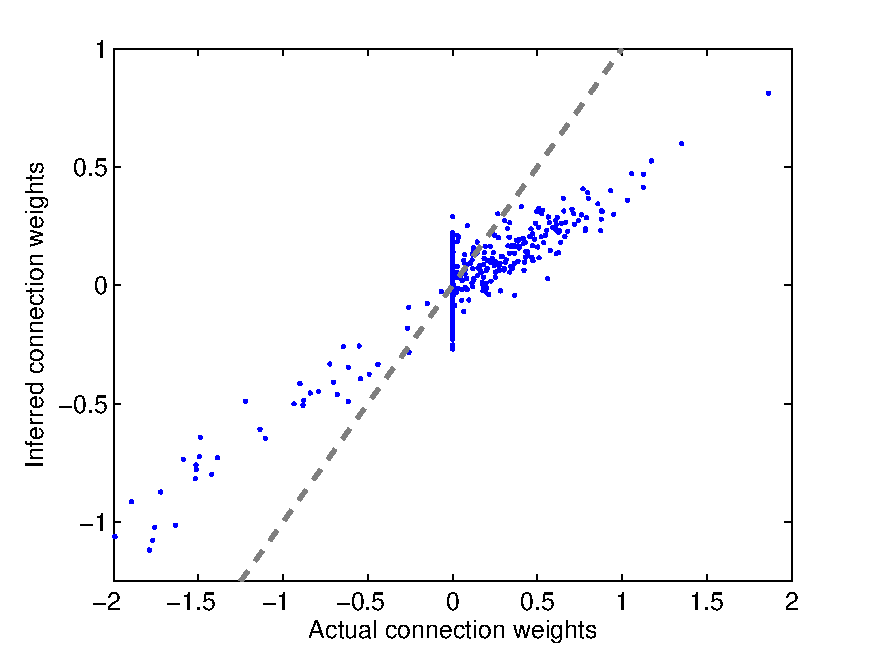
\includegraphics[width=\hsize]{../figs/FigureA8_weak_corr}
\end{minipage}
\begin{minipage}[c]{0.45\hsize}
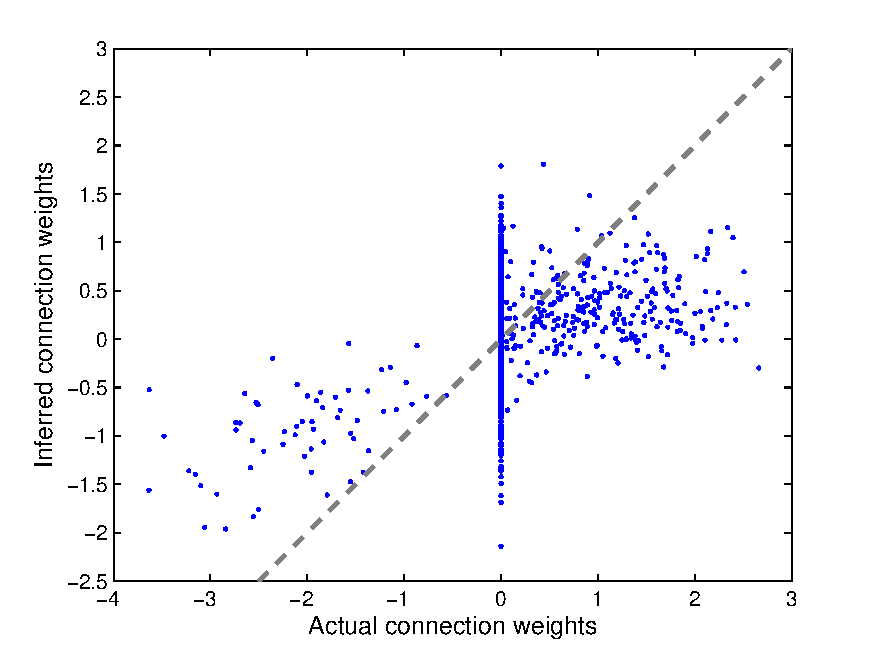
\includegraphics[width=\hsize]{../figs/FigureA8_strong_corr}
\end{minipage}
\caption{
Diverseness of observed neural activity patterns is required for functional connectivity to give access to the actual ``anatomical'' structure of the neural circuit. Here, 15 sec of simulated spike trains for a weakly coupled network (top left panel) and a network with strongly coupled component (top right panel) are shown. In weakly coupled networks, spikes are sufficiently uncorrelated to give access to enough different neural activity patterns to estimate the weights ${\bf w}$. In a strongly coupled case, many highly synchronous events are evident (top right panel), thus preventing observation of sufficiently rich ensemble of activity patterns. Accordingly, the connectivity estimates for the strongly coupled neural network (bottom right panel) does not represent the true connectivity of the circuit, even for the weakly coupled component. This is contrary to the weakly-coupled network (bottom left panel) where true connectivity is successfully obtained. Networks of $N=50$ neurons firing at $\approx 5$ Hz and imaged for $T=10$ min were used to produce this figure.}
\label{fig:rasters}
\end{figure}

On the other hand, our inference algorithm showed significant robustness to deviations of the actual data from our generative model. One important such deviation, which is likely to occur in the real experiments, is variation in the time scales of PSPs in different synapses. Up to now, all PSP time-scales were assumed to be the same in our inference algorithm as well as in the simulations, i.e., $\{\tau^h_{ij}\}_{i,j\leq N}=\tau_h$. In Figure \ref{fig:vartau} we introduce additional variability in $\tau_h$ from one neuron to another. Variability in $\tau_h$ results in added variance in the estimates of the connectivity weights $w_{ij}$ through $\tau_h$ dependence of the scaling factor Eq.~\eqref{eqn:bias}. Still, we found that such added variance was insignificant with $\tau_h$ varying for up to $25\%$ from neuron to neuron.

\begin{figure}[h]
\centering
\begin{minipage}[c]{0.45\hsize}
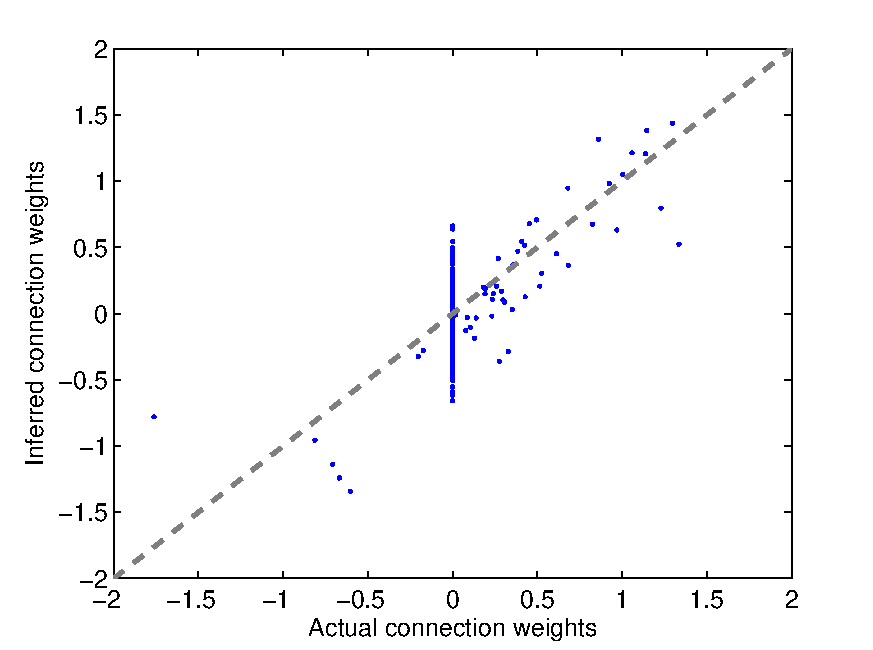
\includegraphics[width=\hsize]{../figs/FigureA9_all_same_sol}
\end{minipage}
\begin{minipage}[c]{0.45\hsize}
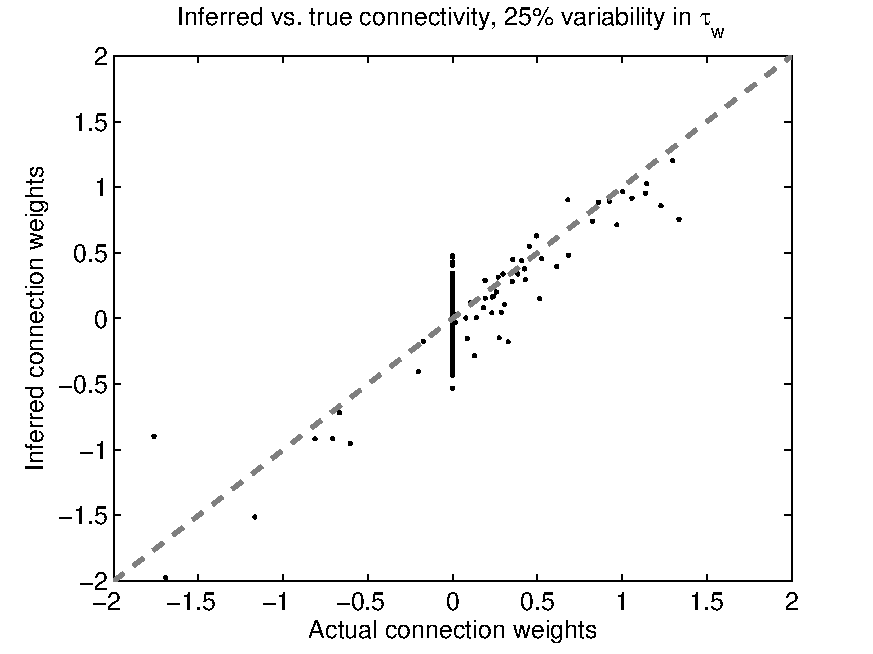
\includegraphics[width=\hsize]{../figs/FigureA9_variable_25}
\end{minipage}
\caption{
Inference is robust to deviations of the data from our generative model. One such deviation, that should be expected in real data, is variability in the PSP time courses from neuron to neuron, and possibly synapse to synapse. With up to $25\%$ variability allowed in PSP time scales $\tau_h$ (right panel), our algorithm provided reconstructions of almost the same quality as when all $\tau_h$'s were the same (left panel). Simulation conditions were the same as in Figure \ref{fig:recvar}.}
\label{fig:vartau}
\end{figure}

%Fig -: real data
% \begin{figure}[h]
% \centering
% \begin{minipage}[c]{0.45\hsize}
% 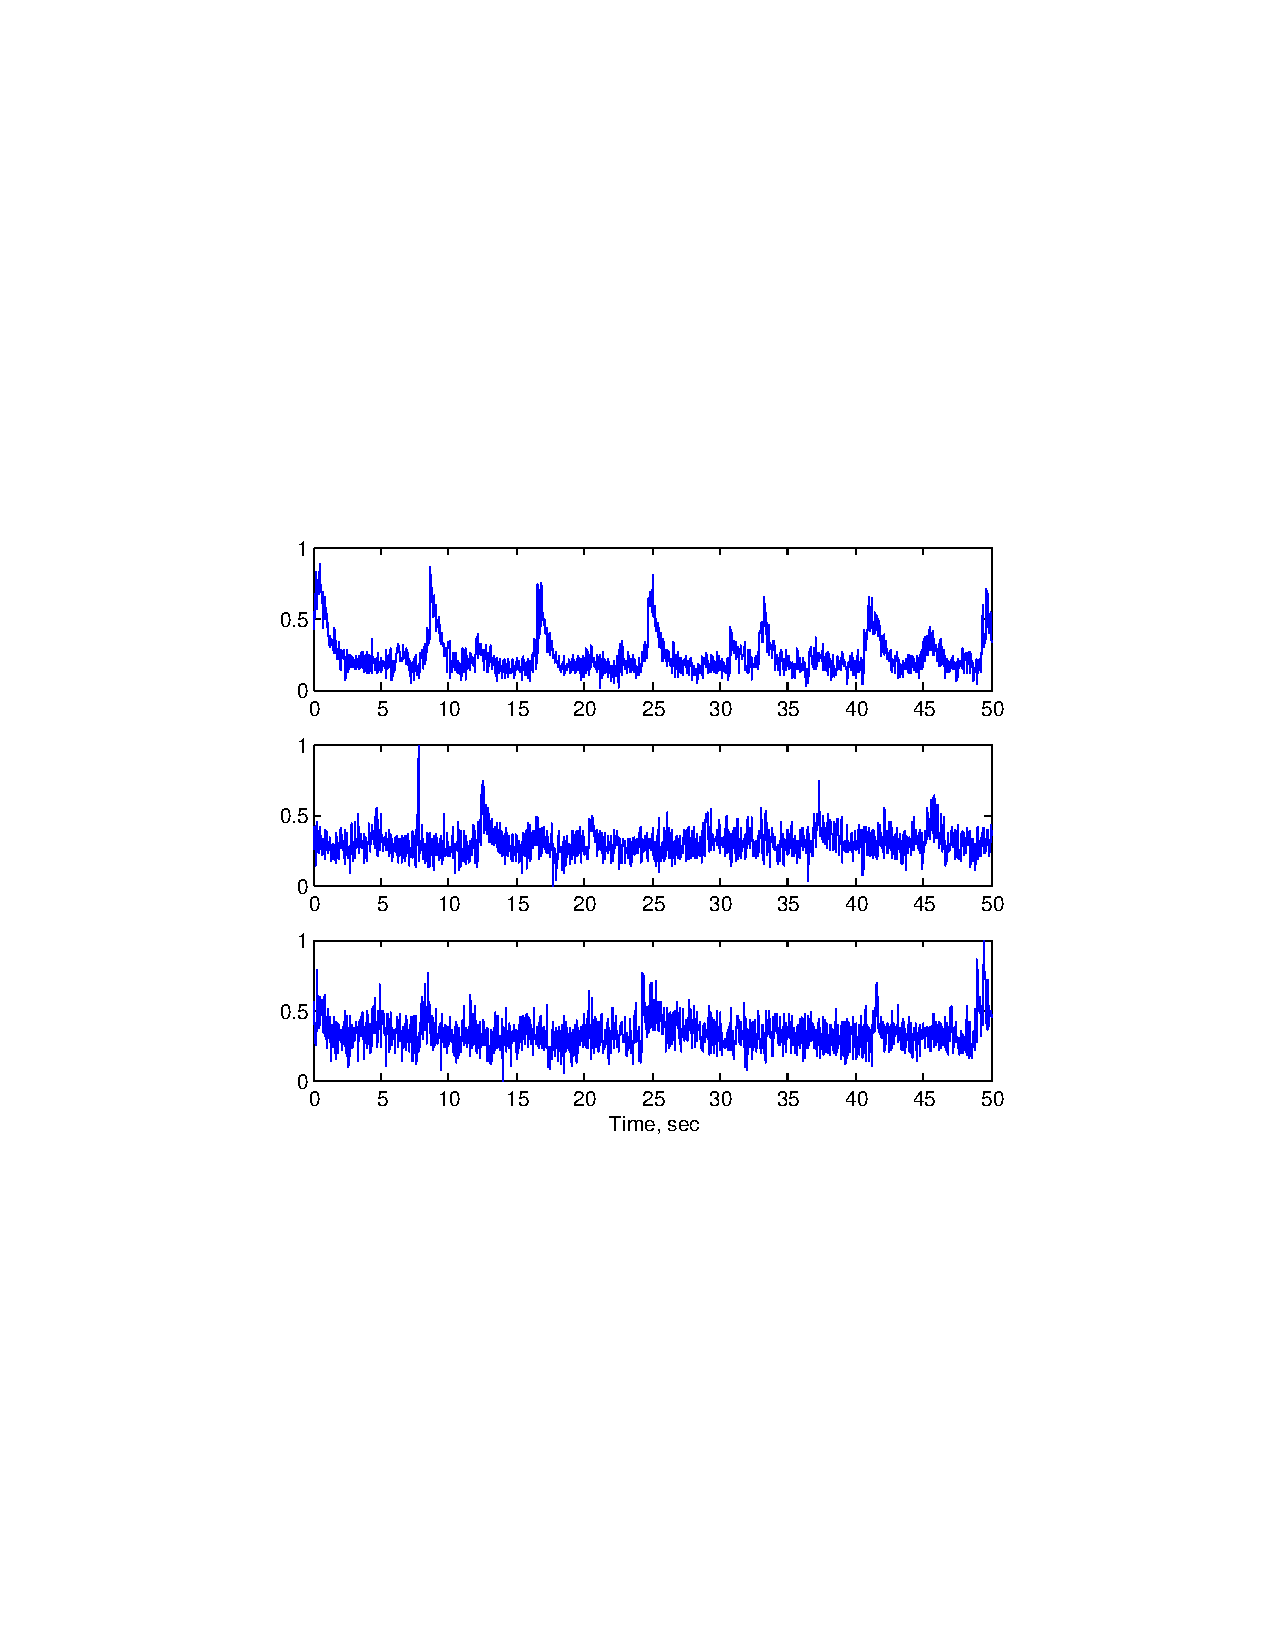
\includegraphics[width=\hsize]{../figs/FigureA11_real_traces}
% \end{minipage}
% \begin{minipage}[c]{0.45\hsize}
% 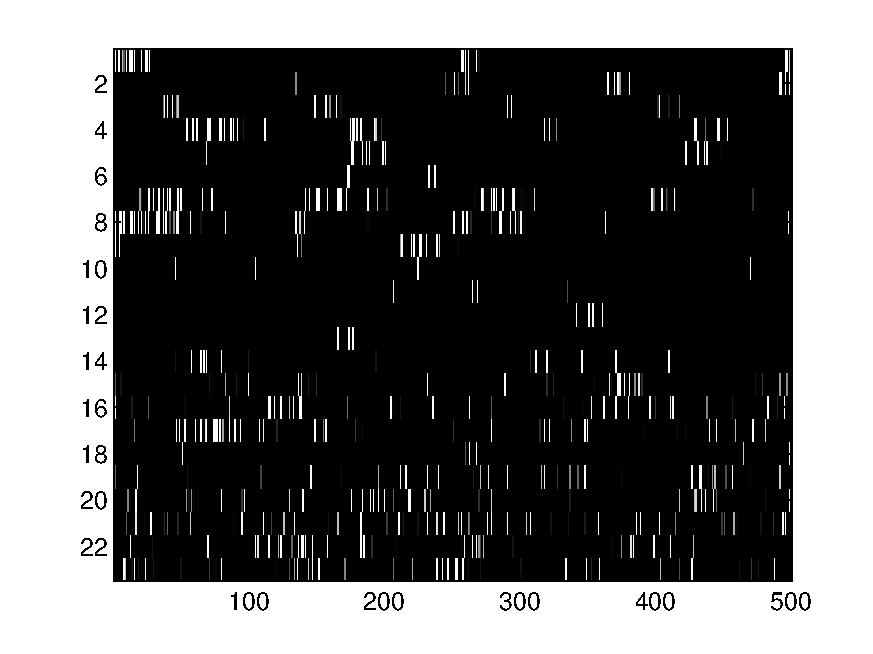
\includegraphics[width=\hsize]{../figs/FigureA11_real_raster}
% \end{minipage}
% \begin{minipage}[c]{0.3\hsize}
% 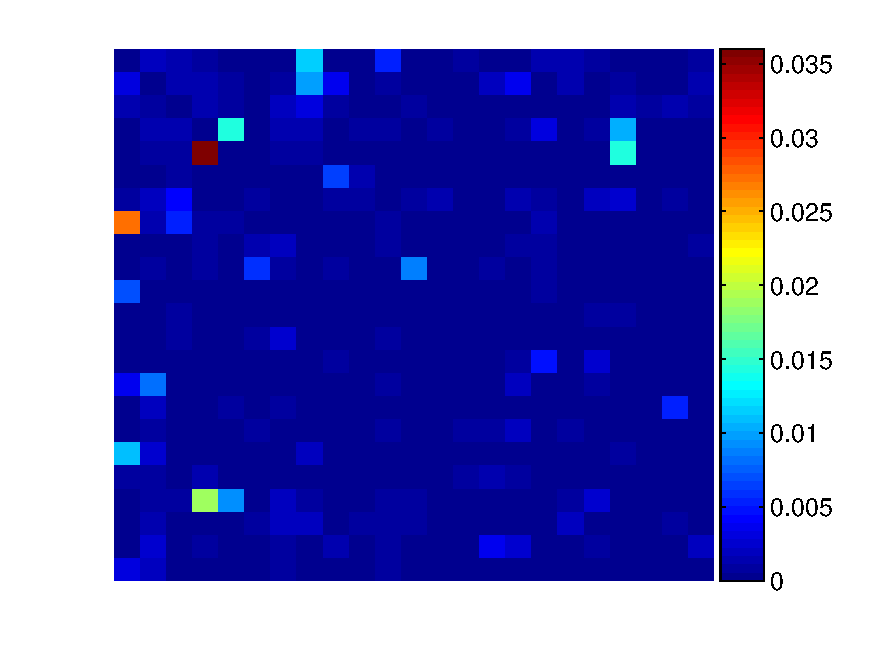
\includegraphics[width=\hsize]{../figs/FigureA11_real_Xcorr}
% \end{minipage}
% \begin{minipage}[c]{0.3\hsize}
% 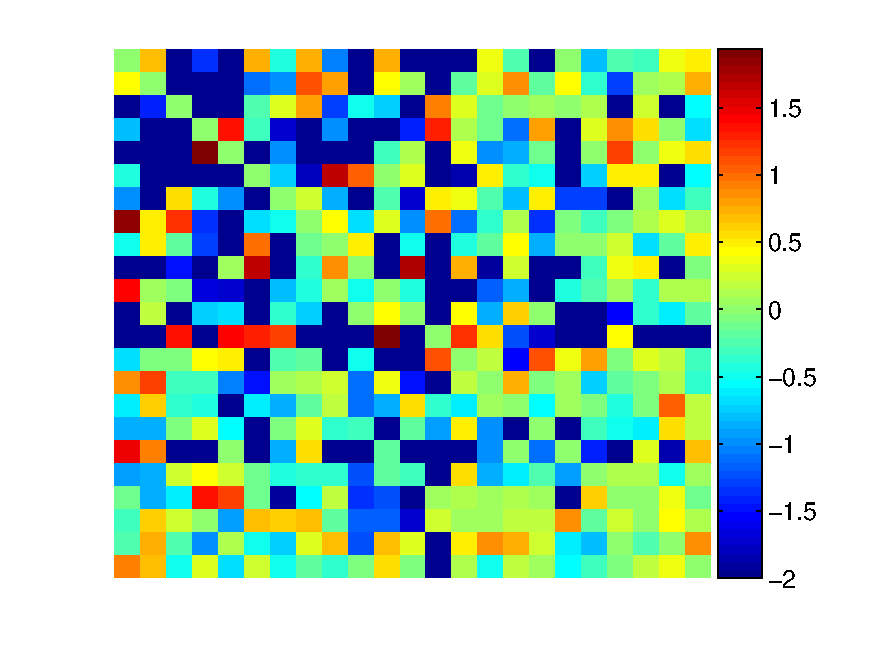
\includegraphics[width=\hsize]{../figs/FigureA11_real_glm}
% \end{minipage}
% \begin{minipage}[c]{0.3\hsize}
% 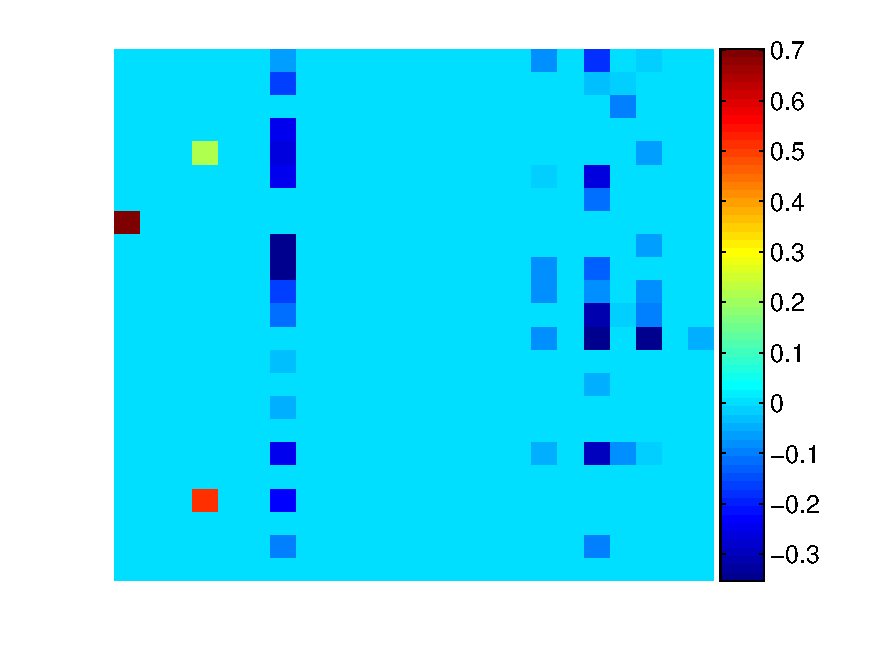
\includegraphics[width=\hsize]{../figs/FigureA11_real_sparse}
% \end{minipage}
% \caption{Functional connectivity matrix inferred from a sample of actual calcium imaging data for $N=72$ cells in [XXX], imaged for $T\approx 260$ sec at 15 Hz.
% $N=23$ neurons with spikes at sufficient SNR were selected, and functional connectivity reconstructed using factorized approximation algorithm. Firing cell of these cells was 0.1-1 Hz and 20-200 spikes were collected for each neuron.
% Upper-left panel shows example of actual fluorescence traces from selected cells, best to worst. Upper-right panel shows a raster of inferred spike trains for first 100 sec of imaging data. Lower panels show left-to-right the time-delayed cross-correlation matrix for selected neurons, simple GLM solution and sparse GLM solution, respectively. A consistent connectivity matrix is obtained here, with sparse solution having sparseness of $\approx 10 \%$, and all neurons automatically respecting Dale's law without explicitly enforcing it. Two clearly excitatory, and three clearly inhibitory neurons can be seen, with remaining neurons not showing significant couplings.}
% \label{fig:real}
% \end{figure}

%We applied our algorithm to a sample of the real calcium imaging data from [XXX], totaling about 5 minutes of imaging for a population of 72 cells in [XXX]. Out of these, about 23 cells had fluorescence traces indicative of spikes, while the other cells were either silent or did not shown SNR sufficient for analysis. These 23 cells were selected for futher processing. 20-200 spikes were found for each cell, corresponding to firing rates from 0.07 Hz to 0.8 Hz.
%We then identified functional connectivity matrix for this population. Sparse solution resulted in consistent connectivity matrix with sparseness of about 10\%, automatically respecting Dale's law, and clearly indicating two strongly connected excitatory neurons and few inihibitory neurons. Although this data lacked independent controls necessary to properly evaluate quality of our obtained reconstruction, it does demonstrate that our approach can be successfully applied under real-life condition to analyze functional connectivity of real populations of neurons.


\section{Discussion}
\label{sec:discussion}
In this paper we develop a partial Bayesian approach for inferring functional connectivity in a population of spiking neurons observed using calcium imaging. While inferring functional connectivity from a set of simultaneous spike train recordings had been previously addressed for micro-electrode techniques \cite{PAN03c, TRUC05}, these approaches assumed observing the ``true'' spike trains of each observable neuron.  However, evidence suggests that even state-of-the-art spike sorting algorithms only obtain approximately $90\%$ accuracy in obtaining spike times \cite{HarrisBuzsaki00, WoodBlack08}.  With that in mind, \cite{Rigat06} developed an approach closely related to that here for such a scenario.  In particular, they also consider a sparse prior, use a Bernoulli GLM model, and develop a Metropolis-within-Gibbs sampler to approximate the necessary sufficient statistics for their model.  To our knowledge, we are the first address the problem of inferring connectivity from calcium population imaging data in a model based approach (though see \cite{Roxin08} for a related issue).  Because calcium imaging, in principle, has capacity to image populations of cells containing $\approx 10^3$--$10^6$ neurons, this opens the way for analysis of micro-circuitry in large and complete populations of neurons in neocortex or other brain areas.

% $\ll$LIAM: Another discussion point: we'll want to discuss the work by fabio rigat specifically: http://ba.stat.cmu.edu/journal/2006/vol01/issue04/rigat.pdf, \cite{Rigat06} \newline they touched on a lot of similar themes: they stress the importance of the prior on the inference (they use a more complicated hierarchical prior for the network structure), they use a bernoulli glm as the foundation of their model, they develop a model to deal with misclassified spikes (they're dealing with noisy multielectrode recordings, but the issues are qualitatively similar to ours), and they end up using metropolis-within-gibbs as their main computational tool. definitely worth checking out if you haven't read this before; we should be careful to cite them where appropriate in the main text, and also discuss the overlap in the discussion.

The main challenge in this problem is indirect nature of calcium imaging data, which provides only noisy, low-pass nonlinear filtered, temporally sub-sampled observations of spikes of individual neurons. In order to find connectivity parameters, in a fully Bayesian settings, the hidden spike trains need to be integrated out. Obtaining a joint sample of unobserved spike trains, needed to compute relevant integrals, is a very non-trivial problem given high dimensionality of the hidden state (which scales at least linearly with $N$). In particular, methods for analyzing calcium imaging data for single neurons, \cite{Vogelstein2009}, do not generalize well for this application. To solve this problem, in this paper we develop a new method for obtaining spike train samples from a population of coupled low-dimensional HMMs by embedding sampling chains of states from individual low-dimensional HMM within a Gibbs sampler that loops in a predefined order over different coupled HMMs. The functional connectivity matrix is then inferred by maximizing the expected value of posterior log-likelihood in EM framework. An exponential prior is used to enforce the sparseness condition of the objective connectivity matrix, which significantly reduces the minimal amount of data required for a particular reconstruction accuracy.

By applying this method to observations of spontaneous activity in a simulated population of neurons, we can efficiently infer the functional connectivity matrix from only $\approx 10$ min of simulated calcium imaging data (c.f Figure \ref{fig:recvar-SNR}, \ref{fig:recvar-NT}). While the embedded-chain-within-Gibbs methods leads to an exact locally MAP estimate, under reasonable calcium imaging conditions we find that significant simplification is possible, where the posterior distribution may be assumed to approximately factorize, $P(\bX|\bF;\theta)\approx \prod P(X_i|F_i;\tilde\theta_i)$. This allows one to obtain samples of joint spike trains much more easily, and in parallel. Since the maximization procedure in EM also can be straightforwardly parallelized, thanks to special structure of the posterior likelihood, the entire inference method can be easily implemented as a highly parallelized application, offering significant savings in data-processing time. If calculations are performed on a large high-performance cluster, reconstruction of the connectivity matrix from $\approx 10$ min of calcium imaging data can be performed nearly in real time, by solving each neuron on a separate node and utilizing only about $10$ minutes of computational time per each node. This is an important virtue of our method.

%And while our estimates exhibit some scale error (c.f. Figure \ref{fig:scatters}), the scale error is explained by the poor temporal resolution inherent in the data (c.f. Figure \ref{fig:bias}).  These results depend on a few theoretical advancements.  First, we develop an embedded-chain-within-blockwise-Gibbs algorithm for jointly sampling spike trains, given the calcium traces. Then, we show that by factorizing, we can obtain approximately equally good estimates (c.f. Figure \ref{fig:scatters}), which greatly expedites the computations.  Finally, we can impose a sparse prior on the connection matrix, justified by recent experimental findings \cite{Chlovksii}, to reduce the amount of observations necessary to obtain good estimates (c.f. Figure \ref{fig:sparse} and \ref{fig:distros}).  And while our approach breaks down in the face of strong correlations (c.f. Figure \ref{fig:rasters}), the algorithm fairs well under certain model misspecifications (c.f. Figure \ref{fig:vartau}).

The above described approach differs significantly from naively computing pairwise measures, such as correlation coefficients, which are far faster to compute.  In particular, our inferred weights depend on \emph{all} the observed neurons, not simply the pairwise measures.  In other words, the sufficient statistic for $\bw_i$ is $P[X_i(t), \bX(t-\Delta) | \bF]$, as compared with correlation-like measures that depend only on $P[X_i(t) | X_j(t-\Delta)]$.  So, while a naive application of correlation coefficients might be attractive here, the resulting estimated ``weights'' are effectively useless (not shown).  

%Our method allows to measure functional connectivity conditioned on the spike trains of all observed neurons, i.e., $(\bn_1,\bn_2 | \bn_3, \ldots, \bn_N)$ \cite{emory, liam, Garofalo, Vakorina, etc.}. This differs significantly from previous works [XXX], which naively defined functional connectivity as a function of spike trains of only two neurons, $(\bn_i,\bn_j)$  - correlation coefficient, lagged cross-correlation, transfer entropy, or Granger causality. Since these measures explicitly ignore the spike trains of all other neurons, they suffer from the problems related to  ``third-neuron-mediated-interactions''. Specifically, if neuron $i$ and neuron $j$ both are strongly connected to third neuron $k$, such naive measures may report strong functional connection between neurons $i$ and $j$, even in the presence of observations of neuron $k$. Our method has added power of resolving such mediated interactions, or ``explaining away'': if correlation between neuron $i$ and neuron $j$ may be successfully modeled by functional connection with the third neuron $k$, our method will ``explain away'' such correlation, and assign to neurons $i$ and $j$ functional connection weight zero. We show that under certain condition (weak correlation among spike trains, c.f. Figure \ref{fig:sparse}) our method allows reconstructing true, ``anatomical'', connectivity matrix for the population of neurons solely from the activity data. At the same time, we demonstrate that under certain conditions such reconstruction from activity data alone may fail: if the spike trains are strongly correlated, functional connectivity matrix may not correspond to the true connectivity of the population even when all neurons are observed (c.f. Figure \ref{fig:rasters}). Such failure can be explained by inability of monitoring neural activity in strongly correlated spike trains to properly sample the space of all activity patterns, necessary to reliably constrain $\bw$.

%Importantly, the above-described approach for learning a functional connection matrix differs significantly from previous work.  Naively, one can define functional connectivity between a pair of neurons as some function of their two spike trains, $f(\bn_1,\bn_2)$.  Examples of such functions include correlation coefficient, lagged cross-correlation, transfer entropy, and Granger causality.  These measures are problematic, in that they implicitly ignore the spike trains of all other neurons.  One would rather have a measure of connectivity that is conditioned on the spike trains of all observable neurons, i.e., $f(\bn_1,\bn_2 | \bn_3, \ldots, \bn_N)$.  Several groups have recently developed methods to infer pairwise connectivity conditioned on all other observable spike trains \cite{emory, liam, Garofalo, Vakorina, etc.}.  To our knowledge, however, this work represents the first attempt to infer connectivity given some data other than spike trains.  As the spikes contain all the information about connectivity, we therefore must infer the spike trains first, and then estimate the functional connectivity.

%In the view of these achievements and failures, 
A number of possible improvements of our method can be proposed. One of the biggest challenges for inferring neural connectivity from functional data is the presence of so called hidden inputs from unobserved neurons \cite{Vidne08}. Since it is typically impossible to expect that activity of all neurons in a closed neural circuit can be monitored, such hidden inputs should be always anticipated in real imaging data. Correlations in hidden inputs are capable of successfully mimicking functional connections among different observed neurons, thus presenting a substantial challenge for estimating neural circuit's connectivity from activity observations alone. Developing methods to cope with such hidden inputs is currently area of active research \cite{Vidne08}.  %Incorporating these features into our model is an important direction for future work. 

Along with investigation of ways to combat the effect of unobserved neurons, we have considered several other potential directions for future improvements of our method.  Incorporating photo-stimulation to activate or deactivate individual neurons or sub-populations may be used to significantly increase statistical power of a given set of observations \cite{Deisseroth05,SzobotaIsacoff07}. %Especially, such external stimulation of network activity may be helpful in the case where the natural activity of a circuit results in strongly correlated firing patterns [Rafa?]. 
Although naturally observed activity may not allow reliable determination of circuit's connectivity matrix, by utilizing external stimulation, a sufficiently rich sample of activity patterns may be collected, and true anatomical structure of the neural circuit may be inferred. Developing the optimal sequences of artificial stimuli and their implementation in the actual experiments are other important directions for future work.

Furthermore, improvements of the algorithms for faster implementation of both the E and M step of our algorithm are under development.  Specifically, fast, non-negative deconvolution of calcium to infer spike trains is a promising alternative \cite{Vogelstein08}.  This fast algorithm utilizes the tridiagonal structure of the state-space problem, a interior-point approach to impose the non-negativity constraint, and Gaussian elimination to ascend the concave likelihood surface in $O(T)$ \cite{Pan08b}.  This approach only yields the MAP estimate of the most likely spike train, and so a true maximization step (integrating over a distribution) is not feasible.  However, approximating the posterior with the MAP seems sufficient when SNR is sufficiently high \cite{Vogelstein08}.

Several improvements in the model are also under investigation.  Explicitly modeling Poisson statistics of the spike counts in time-bins with large width, $\Delta$, rather than Bernoulli distribution used in this work, might helpful for fast spiking neurons. Modifications of our generative model allowing to deal with fluorescent signal non-stationarities, e.g. due to dye bleaching and drift, will be important to reliably apply our method to real data. 

Finally, a fully Bayesian algorithm for estimating the posterior distributions of all the parameters, as opposed to only finding the MAP estimate, is of great interest. Such fully-Bayesian extension is conceptually simple: we just need to extend this work's Gibbs sampler to additionally sample from $\bth$ given the spike trains $\bX$. Since we already have a method for drawing the spike trains $\bX$ given $\bth$ and $\bF$, with such an additional sampler we may obtain samples from $P(\bX,\bth | \bF)$ simply by sampling from $\bX \sim P(\bX|\theta,\bF)$ and $\bth \sim P(\bth |\bX)$ within a Gibbs sampling procedure.  Sampling from the posteriors $P(\bth|\bX)$ in the GLM setting is tractable using hybrid Monte Carlo methods, since all the posteriors are log-concave \cite{Ishwaran99,Gamerman97,Gamerman98,Yashar08}.  All these advances are currently being pursued.

% \begin{acknowledgments}
\section*{Acknowledgements}
The authors would like to acknowledge Rafael Yuste, Brendon O.\ Watson, Adam Packer, Tanya Sippy, Tom Mrsic-Flogel and Vincent Bonin for data and helpful discussions.
% \end{acknowledgments}

\bibliography{mybib}
% \bibliographystyle{amsplain}
\bibliographystyle{apalike}

\end{document} }